\documentclass[fleqn,10pt,aspectratio=169,dvipsnames]{beamer}
\usetheme[
%%% options passed to the outer theme
%    hidetitle,           % hide the (short) title in the sidebar
%    hideauthor,          % hide the (short) author in the sidebar
%    hideinstitute,       % hide the (short) institute in the bottom of the sidebar
%    shownavsym,          % show the navigation symbols
%    width=2cm,           % width of the sidebar (default is 2 cm)
%    hideothersubsections,% hide all subsections but the subsections in the current section
%    hideallsubsections,  % hide all subsections
    right%left               % right of left position of sidebar (default is right)
%%% options passed to the color theme
%    lightheaderbg,       % use a light header background
  ]{AAUsidebar}

%\definecolor{myBlue}{RGB}{52,52,154}

% If you want to change the colors of the various elements in the theme, edit and uncomment the following lines
% Change the bar and sidebar colors:
%\setbeamercolor{AAUsidebar}{fg=myBlue}
%\setbeamercolor{sidebar}{bg=red!20}
% Change the color of the structural elements:
%\setbeamercolor{structure}{fg=red}
% Change the frame title text color:
%\setbeamercolor{frametitle}{fg=blue}
% Change the normal text color background:
%\setbeamercolor{normal text}{bg=gray!10}
% ... and you can of course change a lot more - see the beamer user manual.

\setlength{\mathindent}{0cm}
\usepackage{xcolor}
\usepackage{color}

% A command to highlight stuff
% \highlight[<colour>]{<stuff>}
\newcommand{\highlight}[2][yellow]{\mathchoice%
	{\colorbox{#1}{$\displaystyle#2$}}%
	{\colorbox{#1}{$\textstyle#2$}}%
	{\colorbox{#1}{$\scriptstyle#2$}}%
	{\colorbox{#1}{$\scriptscriptstyle#2$}}}%

% A command to higlight plus name stuff
\definecolor{blueEQ}{RGB}{193, 49, 0}
\definecolor{myGray}{RGB}{84,97,110}
\newlength{\overwritelength}
\newlength{\minimumoverwritelength}
\setlength{\minimumoverwritelength}{0.1cm}
\newcommand{\overwrite}[3][red]{%
	\settowidth{\overwritelength}{$#2$}%
	\ifdim\overwritelength<\minimumoverwritelength%
	\setlength{\overwritelength}{\minimumoverwritelength}\fi%
	\stackrel
	{%
		\begin{minipage}{\overwritelength}%
			\color{#1!40}\centering\tiny #3\\%
			\rule{1pt}{3pt}%
		\end{minipage}}
	{\colorbox{#1!40}{\color{myGray}$\displaystyle#2$}}}

% Trying some videos
\usepackage{multimedia}

%\usepackage[utf8, latin1]{inputenc}
\usepackage[T1]{fontenc}
%\usepackage{fouriernc}

\usepackage[spanish]{babel}
% Or whatever. Note that the encoding and the font should match. If T1
% does not look nice, try deleting the line with the fontenc.
% No indent emunerate
\usepackage{enumitem}
\usepackage{multicol}
\usepackage{wasysym}
%\usepackage{mathpazo}
%\renewcommand\rmdefault{hpv}
%\usepackage{avant}
\usepackage{fontspec}
\usepackage{ragged2e}
\usepackage{color}
\usepackage[customcolors]{hf-tikz}
\usepackage[skins,theorems]{tcolorbox}
\usepackage{mathrsfs,amsmath}
\usepackage{graphicx} 
\usepackage{animate}
\usepackage{multido}
\usepackage{xmpmulti}
%\usepackage{media9}
\usepackage{multimedia}
\usetikzlibrary{positioning, arrows}

\newcommand\scalemath[2]{\scalebox{#1}{\mbox{\ensuremath{\displaystyle #2}}}}
%\usepackage{vwcol} 
%\usepackage{amssymb}
%\tcbset{highlight math style={enhanced, colframe=red,colback=white,arc=0.5pt,boxrule=0.5pt}}

\setmainfont[
Extension=.otf,
UprightFont= *-regular,
BoldFont=*-bold,
ItalicFont=*-italic,
BoldItalicFont=*-bolditalic,
]{texgyreheros}

% Change the font style \rmfamily \normalfont \sffamily
%\renewcommand*\rmdefault{cmss}
%\renewcommand{\familydefault}{\sfdefault}
%\renewcommand{\familydefault}{\rmdefault}

%\usepackage{mathrsfs}
\usefonttheme{professionalfonts}
%\usefonttheme[onlymath]{serif}
%\renewcommand\sfdefault{cmbr}
\usepackage[small,OT1,euler-digits]{eulervm}

% colored hyperlinks
\newcommand{\chref}[2]{%
  \href{#1}{{\usebeamercolor[bg]{AAUsidebar}#2}}%
}


\newcommand\blfootnote[1]{%
	\begingroup
	\renewcommand\thefootnote{}\footnote{#1}%
	\addtocounter{footnote}{-1}%
	\endgroup
}

\usepackage{mathtools}
% et al
\newcommand{\etal}{\textit{et al.}\ }
% Subtitle sze
\setbeamerfont{framesubtitle}{size=\normalsize}
% Num sections in TOC
\setbeamertemplate{section in toc}[sections numbered]

\title[CAO en OCT de fase inestable]{\vspace*{\baselineskip} \LARGE Óptica adaptativa computacional en tomografía de coherencia con sistemas de fase inestable}

\subtitle{\vspace*{.5\baselineskip}\emph{\bf Trabajo de grado I \\ Maestría en Física Aplicada }\vspace*{-.5\baselineskip}} % could also be a conference name


\newif\ifplacelogo % create a new conditional
\placelogotrue % set it to true

\author[Sebastián Ruiz \vspace*{-1.5\baselineskip}]{\bf 
	\vspace*{-2\baselineskip}Sebastián Ruiz Lopera  \vspace*{\baselineskip}\\
	{\small Asesor: Ph.D. René Restrepo Gómez} \\ Área de Instrumentación Óptica Espacial - INTA \vspace*{.5\baselineskip} \\ {\small Co-asesor: Ph.D. Néstor Uribe Paratarroyo} \\ Wellman Center for Photomedicine - MGH - HMS  \vspace*{\baselineskip}\\
	{\footnotesize Escuela de Ciencias \\ Grupo de Óptica Aplicada} \\
	{\footnotesize{13 de febrero de 2020}}\vspace*{-1.5\baselineskip}
}
% - Give the names in the same order as they appear in the paper.
% - Use the \inst{?} command only if the authors have different
%   affiliation. See the beamer manual for an example

%\institute[]{Maestría en Física Aplicada\\Departamento de Ciencias Físicas\\Escuela de Ciencias}

%\date{1 de febrero de 2018} % Nota : Cambiar la fecha
\date{ }

% specify a logo on the titlepage (you can specify additional logos an include them in 
% institute command below
%\pgfdeclareimage[height=1.8cm]{titlepagelogo}{AAUgraphics/aau_logo_new_circle.pdf} % placed on the title page

\pgfdeclareimage[height=1.3cm]{titlepagelogo}{AAUgraphics/logo_eafit_vig_minedu} % placed on the title page

%\pgfdeclareimage[height=1.5cm]{titlepagelogo2}{graphics/aau_logo_new} % placed on the title page
\titlegraphic{% is placed on the bottom of the title page
	\vspace*{-.5\baselineskip}
  \pgfuseimage{titlepagelogo}
%  \hspace{1cm}\pgfuseimage{titlepagelogo2}
}


\begin{document}
% the titlepage
{\aauwavesbg%
\begin{frame}[plain,noframenumbering] % the plain option removes the sidebar and header from the title page
\titlepage
\end{frame}}

%%%%%%%%%%%%%%%%%%%%%%%%%%%   Contenido   %%%%%%%%%%%%%%%%%%%%%%%%%%%%
\begin{comment}
\begin{frame}{Contenido}{}
\large
	\begin{multicols}{2}
\tableofcontents
	\end{multicols}
\end{frame}
\end{comment}
%%%%%%%%%%%%%%%%%%%%%%%%%%%   Introducción OCT  %%%%%%%%%%%%%%%%%%%%%%%%%%%%

\section{Introducción}

\begin{frame}[t]{Introducción}{Tomografía de Coherencia Óptica}
\small
\textbf{Tomografía de Coherencia Óptica (OCT):} Técnica de imagen médica \textit{no--invasiva} para producir imágenes volumétricas de muestras esparsivas e inhomogéneas como los tejidos.
\blfootnote{\tiny{D. Huang \etal \emph{Science,} \textbf{254}: 1178-1181, 1991.}} \blfootnote{\tiny{W. Drexler \etal Optical Coherence Tomography: Technology and Applications. \emph{Springer,} 2015.}}
%\vspace{.75\baselineskip}
	\begin{center}
\includegraphics[height=.58\textheight]{Figures/OCT_Images.pdf}
	\end{center}
\end{frame}

\section{Planteamiento del problema}

\begin{frame}[c]{Planteamiento del problema}
\small
\textbf{OCT es susceptible a aberraciones ópticas:} \\
	\begin{itemize}
\item Propias del sistema óptico,
\item Inducidas por la muestra (e.g. imagen retinal). \\
	\end{itemize}

	\begin{centering}
		\begin{columns}
			\begin{column}{\textwidth}
\hspace*{0\baselineskip}
\includegraphics[width=.47\textwidth]{Figuras/Confocal_gating.png}
\hspace*{.5\baselineskip}
\onslide<2->{\includegraphics[width=.47\textwidth]{Figuras/Human_photoreceptos.png}}
			\end{column}
		\end{columns}
\vspace{\baselineskip}
\onslide<3>{
{\color{red}Compromiso} entre resolución y profundidad de campo. \\
Las aberraciones {\color{red}afectan} la resolución efectiva del sistema. \\
}
	\end{centering}

\blfootnote{\tiny{W. Drexler \etal Optical Coherence Tomography: Technology and Applications. \emph{Springer,} 2015.}}
\blfootnote{\tiny{P. Pande \etal Opt Lett, 41(14): 3324-3327, 2016.}}
%\vspace{.75\baselineskip}
\end{frame}

\begin{frame}[t]{Planteamiento del problema}
La corrección computacional de aberraciones (CAC) es un campo de interés en OCT para evitar o complementar los enfoques basados en \textit{hardware}. CAC opera en el campo complejo con \textbf{modelos analíticos} o \textbf{parámetros derivados de los datos mismos.}
	\begin{center}
		\begin{overprint}
\hspace*{-1\baselineskip}
\onslide<2>\includegraphics[height=.55\textheight]{Figuras/ProblemStatement_1.png}
\onslide<3>\includegraphics[height=.55\textheight]{Figuras/ProblemStatement_2.png}
\onslide<4>\includegraphics[height=.55\textheight]{Figuras/ProblemStatement_3.png}
\onslide<5>\includegraphics[height=.55\textheight]{Figuras/ProblemStatement_4.png}
		\end{overprint}
	\end{center}
\end{frame}

\begin{frame}[t]{Planteamiento del problema}
	\begin{center}
{\onslide<1-> La \textbf{corrección de aberraciones} es de gran interés para potenciar el desempeño de OCT al obtener imágenes que preservan la información de estructuras finas, así como para extender el DOF en imágenes de alta resolución. \\}

\vspace{\baselineskip}
{\onslide<2->Las \textbf{técnicas computacionales} operan con el {\color{blue}campo complejo}, por lo que requieren \textit{estabilidad de fase}, que {\color{red}solo se obtiene en sistemas con configuraciones especificas, limitando su aplicabilidad.} \\}

\vspace{\baselineskip}		
{\onslide<3-> Se propone desarrollar una {\color{blue}estrategia computacional de corrección de aberraciones ópticas} en tomografía de coherencia óptica que pueda {\color{blue}operar en sistemas sin estabilidad de fase}, ampliando así la aplicabilidad de estas técnicas en sistemas más comunes, {\color{blue}sin configuraciones especificas.} \\}
	\end{center}
\end{frame}

%%%%%%%%%%%%%% Marco teórico
\section{Marco teórico}

\begin{frame}[t]{Marco teórico}{Modelo de la señal de OCT}
OCT se puede considerar con un problema de scattering inverso:
\vspace{\baselineskip}
	\begin{columns}
		\begin{column}{.4\textwidth}
			\begin{center}
				\begin{overprint}
\onslide<1>\includegraphics[height=.5\textheight]{Figuras/Theory_ConvModel_1.png}
\onslide<2->\includegraphics[height=.5\textheight]{Figuras/Theory_ConvModel_2.png}
				\end{overprint}
			\end{center}
		\end{column}
		\begin{column}{.6\textwidth}
\small
{\onslide<2-> Se mide el {\color{red}\textit{scattering} $S(x, y; k)$} pero se desea el potencial del  {\color{blue}\textit{scatter} $\eta(x, y; z)$} que lo produjo: $${\color{red}S(x, y; k)} = {\color{ForestGreen}h(x, y, z; k)}\ast {\color{blue}\eta(x, y, z)}$$ $${\color{red}\tilde{S}(q_x, q_y; k)} = {\color{ForestGreen}H(q_x, q_y; k)}{\color{blue}\tilde{\tilde{\eta}}(q_x, q_y, q_z)},$$
}
{\onslide<3->donde $(x, y, z)$ y $(q_x, q_y, q_z)$ son las coordenadas espaciales y frecuenciales respectivamente, {\color{ForestGreen}$h(x, y, z; k)$} es la función respuesta al impulso, {\color{ForestGreen}$H(q_x, q_y; k)$} es la función de transferencia óptica, y los operadores $\tilde{f}$ y $\tilde{\tilde{f}}$ representan la transformada de Fourier 2D y 3D de la función $f$. \\
}
{\onslide<4->\vspace{\baselineskip}
Se captura {\color{red}$S(x, y; k)$} y computacionalmente se revierte el efecto de {\color{ForestGreen}$h(x, y, z; k)$} para recuperar {\color{blue}$\eta(x, y, z)$}.
}
		\end{column}
	\end{columns}
\end{frame}

\begin{frame}[c]{Marco teórico}{Corrección computación de aberraciones en OCT}
	\begin{columns}
		\begin{column}{.74\textwidth}
{\footnotesize
{\onslide<1->Procesamiento basado en el \textbf{campo complejo} $\rightarrow {\color{red}A}\exp\{i{\color{blue}\phi}\}$ ({\color{red}amplitud} y {\color{blue}fase}).
Intensidad ${\color{red}A}\exp\{i{\color{blue}\phi}\}|^2 = |{\color{red}A}|^2 \rightarrow$ Imagen estructural no depende de la fase. \\
}

\vspace{\baselineskip}
Para CAC \textbf{se requiere estabilidad de fase} $\rightarrow$ \textit{relación coherente entre la medida en una posición y otra.} \\
\vspace{\baselineskip}
			\begin{itemize}
\item \textbf{Sistemas de campo completo:} fase estable en todo el {\color{ForestGreen}volumen (3D)}. \\
\item \textbf{Sistemas de escaneo puntual:} fase estable dentro de \textit{A-lines} ({\color{red}axial 1D}) o dentro de \textit{B-scans} ({\color{red}corte transversal 2D}). \\
			\end{itemize}
}
		\end{column}
	\begin{column}{.25\textwidth}
\includegraphics[width=\textwidth]{Figuras/Scanning_point.png}
	\end{column}
	\end{columns}
{\small
	\vspace{\baselineskip}
\textbf{Causas de inestabilidades de fase:}
	\begin{columns}
		\begin{column}{.5\textwidth}
			\begin{itemize}
\item Debido a la muestra: \\
\hspace{.5\baselineskip} Movimiento de cuerpo rígido. \\
\hspace{.5\baselineskip} Movimiento Browniano.
			\end{itemize}
		\end{column}
		\begin{column}{.5\textwidth}
			\begin{itemize}
\item Debido a al sistema: \\ 
\hspace{.5\baselineskip} Sistema de escaneo. \\
\hspace{.5\baselineskip} Sistema de adquisición de la señal.
			\end{itemize}
		\end{column}
	\end{columns}
}
\blfootnote{\tiny{N.D. Shemonski \etal \emph{Opt Express,} \textbf{22}: 19183-19197, 2014.}}
\end{frame}

\begin{frame}[c]{Marco teórico}{Configuraciones experimentales}
	\begin{overprint}
\hspace{-\baselineskip}
\onslide<1>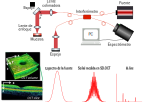
\includegraphics[height=.5\textheight]{Figuras/SD-OCT.png}
\onslide<2>\includegraphics[height=.5\textheight]{Figuras/FF-SSOCT_1.png}
\onslide<3->\includegraphics[height=.5\textheight]{Figuras/FF-SSOCT_2.png}
	\end{overprint}
	\begin{centering}
{\onslide<3->
{\small CAC opera en sistemas de \textbf{\textit{Spectral-Domain} OCT} y en \textbf{\textit{Full-Field Swept-Source} OCT}. \\
}
}
{\onslide<4->\textbf{{\color{red}No opera}} con \textit{Swept-Source} OCT de escaneo puntual. \\
}
	\end{centering}

\end{frame}

\begin{frame}[c]{Marco teórico}{\text{Swept-Soure OCT}}
	\begin{overprint}
\onslide<1>\includegraphics[width=\textwidth]{Figuras/SSOCT_Jitter_1}
\onslide<2>\includegraphics[width=\textwidth]{Figuras/SSOCT_Jitter_2}
\onslide<3>\includegraphics[width=\textwidth]{Figuras/SSOCT_Jitter_3}
\onslide<4>\includegraphics[width=\textwidth]{Figuras/SSOCT_Jitter_4}
\onslide<5>\includegraphics[width=\textwidth]{Figuras/SSOCT_Jitter_5}
\onslide<6>\includegraphics[width=\textwidth]{Figuras/SSOCT_Jitter_6}
\onslide<7->\includegraphics[width=\textwidth]{Figuras/SSOCT_Jitter_7}
	\end{overprint}

\vspace{\baselineskip}
{\onslide<8>
	\begin{centering}
$S^\ast (x, y; z) = S(x, y; z) \exp\{i\beta_0z\}$ \\
$\beta_0 = \beta_0(x, y)$ \\
	\end{centering}
}
\end{frame}

\begin{frame}[c]{Marco teórico}{\text{Swept-Soure} OCT}

\onslide<1->\includegraphics[width=.32\textwidth]{Figuras/Phase_example_1.pdf}
\onslide<2->\includegraphics[width=.32\textwidth]{Figuras/Phase_example_2.pdf}
\onslide<3->\includegraphics[width=.32\textwidth]{Figuras/Phase_example_3.pdf}

\vspace{\baselineskip}
	\begin{centering}
En medios esparsivos como el tejido, la imagen coherente produce \textbf{speckle}.
La fase del speckle es \textit{aleatoria pero suave} y coherente dentro del tamaño de este. \\
	\end{centering}
\end{frame}

\begin{comment}

%%%%%%%%%%%%%%%%%%%%%%%%%%%   Introducción SD-OCT 1  %%%%%%%%%%%%%%%%%%%%%%%%%%%%

\begin{frame}[t]{Introducción}{Tomografía de coherencia óptica en el dominio del tiempo}
\small
\textbf{Tomografía de coherencia óptica (OCT):} Interferometría de baja coherencia (con una fuente de espectro ancho). \blfootnote{\tiny{C. Dorrer \etal\emph{J. Opt. Soc. Am. B,} \textbf{17}: 1795-1902, 2000.}}
\vspace{-1.5\baselineskip}
	\begin{columns}
		\begin{column}{.65\textwidth}
			\begin{figure}[!ht]
\hspace*{.01\textwidth}
\includegraphics[height=.57\textheight]{Figures/SD-OCT_0.pdf}
			\end{figure}
		\end{column}%
\hspace*{.05\textwidth}
		\begin{column}{.3\textwidth}
\small
		\end{column}
	\end{columns}

\end{frame}

%%%%%%%%%%%%%%%%%%%%%%%%%%%   Introducción SD-OCT 2  %%%%%%%%%%%%%%%%%%%%%%%%%%%%

\begin{frame}[t]{Introducción}{Tomografía de coherencia óptica en el dominio espectral}
\small
\textbf{Tomografía de coherencia óptica en el dominio espectral (SD--OCT):} captura la intensidad de la interferencia en el {\color{blue}dominio de frecuencias} con un {\color{blue}espectrómetro}. \blfootnote{\tiny{C. Dorrer \etal\emph{J. Opt. Soc. Am. B,} \textbf{17}: 1795-1902, 2000.}}
\vspace{-1.5\baselineskip}
	\begin{columns}
		\begin{column}{.65\textwidth}
			\begin{figure}[!ht]
\hspace*{.01\textwidth}
				\begin{overprint}
\onslide<1>\includegraphics[height=.57\textheight]{Figures/SD-OCT_1.pdf}
\onslide<2>\includegraphics[height=.57\textheight]{Figures/SD-OCT_2.pdf}
\onslide<3>\includegraphics[height=.57\textheight]{Figures/SD-OCT_2.pdf}
\onslide<4>\includegraphics[height=.57\textheight]{Figures/SD-OCT_3.pdf}
\onslide<5->\includegraphics[height=.57\textheight]{Figures/SD-OCT_4.pdf}
				\end{overprint}
			\end{figure}
		\end{column}%
\hspace*{.05\textwidth}
		\begin{column}{.3\textwidth}
			\begin{itemize}
\small
\vspace*{\baselineskip}
\item<2-> Interferencia en el dominio de la {\color{blue}longitud de onda}. \\
\vspace{.5\baselineskip}
\item<3-> {\color{blue}Incrementar el muestreo}. \\
\vspace{.5\baselineskip}
\item<4-> {\color{blue}Interpolar} el espectro de $\lambda$ a $k$. \\
\vspace{.5\baselineskip}
\item<5-> {\color{blue}Transformada de Fourier} para obtener la reflectividad. \\
			\end{itemize}
		\end{column}
	\end{columns}
\end{frame}

%%%%%%%%%%%%%%%%%%%%%%%%%%%   Planteamiento del problema  %%%%%%%%%%%%%%%%%%%%%%%%%%%%

\subsection{Planteamiento del problema}

\begin{frame}[c]{Planteamiento del problema}
	\begin{center}
\Large
\onslide<1->{
	Los cálculos numéricos {\color{red}consumen tiempo} y aumentan la {\color{red}caída de la sensibilidad} de la señal con la profundidad\\ (\textit{sensitivity fall--off}).\\
	\vspace{\baselineskip}
}

\onslide<2->{
	{\color{blue}Emplear un espectrómetro lineal en el número de onda.} \\
	\vspace{\baselineskip}
}

\onslide<3->{
	Diseño e implementación a nivel de laboratorio de un espectrómetro que cumpla los requerimientos de la técnica que pueda ser integrado en un futuro sistema de SD--OCT.
}

\blfootnote{\tiny{V.M. Gelikonow \etal \emph{Optics and Spectroscopy}. 106:459--465, 2009.}}
\blfootnote{\tiny{S.W. Lee \etal \emph{Journal of the Optical Society of Korea}. 19:55--62, 2015.}} \blfootnote{\tiny{G. Lan \etal \emph{Scientific Reports,} \textbf{7}:42353, 2017.}}
	\end{center}
\end{frame}

%%%%%%%%%%%%%%%%%%%%%%%%%%%   Objetivos  %%%%%%%%%%%%%%%%%%%%%%%%%%%%

\subsection{Objetivos}

\begin{frame}[c]{Objetivos}
	\begin{center}

\onslide<1->{
Diseñar e implementar un {\color{blue}espectrómetro} usando una red de difracción para ser usado en la técnica de {\color{blue}tomografía de coherencia óptica de segunda generación} a nivel de laboratorio.
	\vspace{\baselineskip}
}

\onslide<2->{
		\begin{itemize}
\item Evaluar {\color{blue}configuraciones} de espectrómetros.
\vspace{.5\baselineskip}

\item Caracterizar la respuesta de la  {\color{blue}cámara CCD}.
\vspace{.5\baselineskip}	

\item Diseñar un {\color{blue}sistema óptico} en OpticStudio.
\vspace{.5\baselineskip}

\item Realizar un {\color{blue}montaje} a nivel de laboratorio.
\vspace{.5\baselineskip}

\item Diseñar el {\color{blue}sistema opto-mecánico} que permita la alineación del espectrómetro.
\vspace{.5\baselineskip}

\item Analizar los {\color{blue}efectos mecánicos} sobre los componentes ópticos.
		\end{itemize}
}
	\end{center}
\end{frame}


%%%%%%%%%%%%%%%%%%%%%%%%%%%   Aspectos teóricos y prácticos   %%%%%%%%%%%%%%%%%%%%%%%%%%%%

\section{Aspectos teóricos y prácticos}

%%%%%%%%%%%%%%%%%%%%%%%%%%%   Contenido   %%%%%%%%%%%%%%%%%%%%%%%%%%%%
\begin{frame}{Contenido}{}
	\begin{multicols}{2}
\tableofcontents[currentsection]
	\end{multicols}
\end{frame}

%%%%%%%%%%%%%%%%%%%%%%%%%%%   Interferometría de baja coherencia   %%%%%%%%%%%%%%%%%%%%%%%%%%%%

\subsection{Marco teórico SD-OCT}
\begin{frame}{Aspectos teóricos y prácticos}{Interferometría de baja coherencia}
	\begin{overprint}
\hspace*{.1\textwidth}
\onslide<1>\includegraphics[height=.8\textheight]{Figures/SD-OCT_Scheme_1.pdf}
\onslide<2>\includegraphics[height=.8\textheight]{Figures/SD-OCT_Scheme_2.pdf}
\onslide<3>\includegraphics[height=.8\textheight]{Figures/SD-OCT_Scheme_3.pdf}
\onslide<4>\includegraphics[height=.8\textheight]{Figures/SD-OCT_Scheme_4.pdf}
\onslide<5>\includegraphics[height=.8\textheight]{Figures/SD-OCT_Scheme_5.pdf}
\onslide<6>\includegraphics[height=.8\textheight]{Figures/SD-OCT_Scheme_6.pdf}
\onslide<7>\includegraphics[height=.8\textheight]{Figures/SD-OCT_Scheme_7.pdf}
\onslide<8>\includegraphics[height=.8\textheight]{Figures/SD-OCT_Scheme_8.pdf}

	\end{overprint}
\end{frame}


%%%%%%%%%%%%%%%%%%%%   Interferometría de baja coherencia en el dominio de Fourier 2   %%%%%%%%%%%%%%%%%%%%

\begin{frame}[c]{Aspectos teóricos y prácticos}{Interferometría de baja coherencia en el dominio de Fourier}
	\begin{center}
		\begin{overprint}
\onslide<1> \includegraphics[height=.8\textheight]{Figures/FD-OCT_A-line_2.pdf}
\onslide<2> \includegraphics[height=.8\textheight]{Figures/FD-OCT_A-line_3.pdf}
		\end{overprint}
	\end{center}
\end{frame}

%%%%%%%%%%%%%%%%%%%%%%%%%%%   Parametros practicos   %%%%%%%%%%%%%%%%%%%%%%%%%%%%

\begin{frame}[t]{Aspectos teóricos y prácticos}{Parámetros prácticos en SD--OCT}
\blfootnote{\tiny{W. Drexler \etal Optical Coherence Tomography: Technology and Applications. \emph{Springer,} 2015.}}
\blfootnote{\tiny{S.W. Lee \etal \emph{Journal of the Optical Society of Korea}. 55:2354, 2009.}}

\vspace{-2\baselineskip}
	\begin{columns}
		\begin{column}{.5\textwidth}
\onslide<1->{
			\begin{equation*}
\textbf{Resolución axial: } \Delta z = 	{\color{PineGreen}\zeta}\frac{2\ln2}{\pi}\frac{{\color{blue}\lambda_0}}{{\color{red}\Delta\lambda}}
			\end{equation*}
			\begin{align*}
{\color{PineGreen}\zeta}\ &:\ \text{Factor de forma.} \\
{\color{blue}\lambda_0}\ &:\ \text{Longitud de onda central.} \\
{\color{red}\Delta\lambda}\ &:\ \text{Ancho espectral a la mitad del máximo.}
			\end{align*}
}

\vspace{-2\baselineskip}
%\onslide<2->{
%			\begin{equation*}
%\textbf{Resolución lateral: }\Delta x = \frac{2{\color{blue}\lambda_0}}{\pi}\frac{1}{{\color{Goldenrod}NA}}
%			\end{equation*}
%			\begin{align*}
%{\color{Goldenrod}\text{NA}}=\frac{D}{2f}\ &:\ \text{Apertura númerica.} \\
%			\end{align*}
%}

		\end{column}
		\begin{column}{.5\textwidth}
\vspace{1.5\baselineskip}
\onslide<2->{
			\begin{equation*}
	\textbf{Rango máximo: }z_{\text{max}} = \frac{\pi}{2{\color{YellowOrange}\delta k}}
			\end{equation*}
			\begin{align*}
{\color{YellowOrange}\delta k}=\frac{2\pi{\color{Emerald}\Delta\lambda_{full}}}{{\color{RubineRed}N}{\color{blue}\lambda_0}^2}\ &:\ \text{Resolución espectral.} \\
{\color{RubineRed}N}\ &:\ \text{Número de píxeles}. \\
{\color{Emerald}\Delta\lambda_{full}}\ &:\ \text{Rango espectral.}
			\end{align*}
}
\vspace{-\baselineskip}
\onslide<3->{
			\begin{equation*}
\textbf{Criterio de Nyquist: } \frac{2\pi}{\color{YellowOrange}\delta k} \leq N \Delta z
			\end{equation*}
			\begin{align*}
{\color{Emerald}\Delta\lambda_{full}} \geq {\color{PineGreen}\zeta} \frac{\pi}{2\ln2} {\color{red}\Delta\lambda}
			\end{align*}
}
		\end{column}
	\end{columns}
\vspace{-\baselineskip}
\end{frame}

%%%%%%%%%%%%%%%%%%%%%%%%%%%   Espectrómetros dispersivos   %%%%%%%%%%%%%%%%%%%%%%%%%%%%

\subsection{Espectrómetros dispersivos}

\begin{frame}{Aspectos teóricos y prácticos}{Espectrómetros dispersivos}
\blfootnote{\tiny{W. Neumann. Fundamentals of Dispersive Optical Spectroscopy Systems. \emph{SPIE Press,} 2015.}}
	\begin{columns}
\hspace{\baselineskip}
		\begin{column}{.65\textwidth}
\includegraphics[width=\textwidth]{Figures/SpecConfig.pdf}
		\end{column}
	
		\begin{column}{.4\textwidth}
\only<2,3,4,5>{
\small
\vspace{-2\baselineskip}
			
Elemento dispersor:\\
%\vspace{\baselineskip}
			\begin{itemize}
\item<2-> Red de difracción
\item<3-> Prisma dispersivo.
\item<4-> Combinación de ambos
			\end{itemize}
\vspace{-.5\baselineskip}
\onslide<5->\hspace{.75\baselineskip}$\rightarrow$ Espectro equidistante en $k$.
}
		\end{column}
	\end{columns}
\end{frame}

%%%%%%%%%%%%%%%%%%%%%%%%%%%   Red de difracción 3   %%%%%%%%%%%%%%%%%%%%%%%%%%%%

\begin{frame}[c]{Aspectos teóricos y prácticos}{Red de difracción}
\blfootnote{\tiny{E. Hecht. Optics. \emph{Pearson Education,} 2017.}}
	\begin{columns}
		\begin{column}{.65\textwidth}
\includegraphics[width=\textwidth]{Figures/DiffractionGrating.pdf}
		\end{column}
		\begin{column}{.3\textwidth}
\onslide<2->{
\textbf{Ecuación de la red de difracción:}
\vspace{-.5\baselineskip}
			\begin{equation*}
\sin\theta_i\pm\sin\theta_{d_m}=md\lambda 
			\end{equation*}
}
\onslide<3->{
\textbf{Rango espectral libre:}\\
\vspace{-\baselineskip}
			\begin{equation*}
\Delta\lambda_{FSR} = \frac{\lambda}{m}
			\end{equation*}
}
\onslide<4->{
\textbf{Dispersión angular:}\\
\vspace{-\baselineskip}
			\begin{equation*}
\frac{\delta\theta_{d_m}}{\delta\lambda} = \frac{md}{\cos\theta_{d_m}}
			\end{equation*}
}
		\end{column}
	\end{columns}
\end{frame}

%%%%%%%%%%%%%%%%%%%%%%%%%%%   Prisma dispersivo 1   %%%%%%%%%%%%%%%%%%%%%%%%%%%%

\begin{frame}[c]{Aspectos teóricos y prácticos}{Prisma dispersivo}
\blfootnote{\tiny{E. Hecht. Optics. \emph{Pearson Education,} 2017.}}
	\begin{center}
\includegraphics[width=.85\textwidth]{Figures/PrismEquation.pdf}
\vspace{\baselineskip}
		\begin{equation*}
\hspace{.25\textwidth}
\theta_{t_2}(\lambda) = \arcsin\bigg(n(\lambda)\sin\bigg[\alpha - \arcsin\bigg( \frac{\sin\theta_{i_1}}{n(\lambda)} \bigg)\bigg]\bigg)
		\end{equation*}
	\end{center}
\end{frame}

%%%%%%%%%%%%%%%%%%%%%%%%%%%   Diseño óptico   %%%%%%%%%%%%%%%%%%%%%%%%%%%%

\section{Diseño óptico}

%%%%%%%%%%%%%%%%%%%%%%%%%%%   Contenido   %%%%%%%%%%%%%%%%%%%%%%%%%%%%
\begin{frame}{Contenido}{}
	\begin{multicols}{2}
\tableofcontents[currentsection]
	\end{multicols}
\end{frame}

%%%%%%%%%%%%%%%%%%%%%%%%%%%   Consideraciones iniciales 1   %%%%%%%%%%%%%%%%%%%%%%%%%%%%

\subsection{Consideraciones iniciales}
\begin{frame}{Diseño óptico}{Consideraciones iniciales}
	\begin{columns}
		\begin{column}{.5\textwidth}
\onslide<2-> \textbf{Fuente de iluminación: } \\ Lámpara halógena de alta potencia (500~mW) con filtro espectral: \\ 
\onslide<3->{
$\Delta\lambda$ = 120~nm @ 840~nm $\rightarrow$ 3.05~$\mu$m.
}
\onslide<4->{
			\begin{columns}
				\begin{column}{.5\textwidth}
					\begin{align*}
\Delta_{\lambda_{full}} &= \zeta\frac{\pi}{2\ln2}\Delta\lambda \\
& = 160nm
					\end{align*}
				\end{column}
				\begin{column}{.5\textwidth}
					\begin{align*}
z_{max} &= \frac{N\lambda_0}{4\Delta\lambda_{full}} \\
&= 2.01 mm
					\end{align*}
				\end{column}
			\end{columns}
		}
		\end{column}
		\begin{column}{.5\textwidth}
\onslide<5->\textbf{Detector: } 
			\begin{itemize}
\item<6-> 2048 x 4 píxeles (14x56~$\mu$m).
\item<7-> Respuesta espectral ente 350--1100nm.
\item<8-> Resolución A/D de 16 bits.
\item<9-> Tiempo de integración entre 1.054~ms--50s (máx. 900Hz).
			\end{itemize}
		\end{column}
	\end{columns}
\end{frame}


%%%%%%%%%%%%%%%%%%%%%%%%%%%   Configuración óptica   %%%%%%%%%%%%%%%%%%%%%%%%%%%%

\subsection{Configuración óptica}

\begin{frame}[t]{Diseño óptico}{Configuración óptica}
	\begin{columns}
		\begin{column}{\textwidth}
			\begin{overprint}
%\vspace*{-2\baselineskip}
\hspace*{.025\textwidth}
%\onslide<1>\includegraphics[width=.9\textwidth]{Figures/Spectrometer_layout_6.pdf}
\onslide<2>\includegraphics[height=.75\textheight]{Figures/Spectrometer_layout_1.pdf}
\onslide<3>\includegraphics[height=.75\textheight]{Figures/Spectrometer_layout_2.pdf}
\onslide<4>\includegraphics[height=.75\textheight]{Figures/Spectrometer_layout_3.pdf}
\onslide<5>\includegraphics[height=.75\textheight]{Figures/Spectrometer_layout_4.pdf}
\onslide<6>\includegraphics[height=.75\textheight]{Figures/Spectrometer_layout_5.pdf}
\onslide<7>\includegraphics[height=.75\textheight]{Figures/Spectrometer_layout_6.pdf}
			\end{overprint}
		\end{column}
\hspace*{-.4\textwidth}
		\begin{column}{.5\textwidth}
			\begin{itemize}
\vspace*{-8\baselineskip}
\small
\item<2-> Acoplador de fibra óptica (NA 0.13).
\item<3-> Espejo parabólico a 90$^\circ$.
\item<4-> Red de difracción a transmisión.
\item<5-> Prisma triangular equilatero.
\item<6-> Doblete acromático.
\item<7-> Cámara lineal (2048 pixels).
			\end{itemize}
		\end{column}
	\end{columns}
\end{frame}

%%%%%%%%%%%%%%%%%%%%%%%%%%%   Sistema de colimación   %%%%%%%%%%%%%%%%%%%%%%%%%%%%

%\subsection{Sistema de colimación}
\begin{frame}{Diseño óptico}{Sistema de colimación}
\includegraphics[width=\textwidth]{Figures/Collimator_comparision.pdf}
\end{frame}

%%%%%%%%%%%%%%%%%%%%%%%%%%%   Selección del grupo de dispersión 1   %%%%%%%%%%%%%%%%%%%%%%%%%%%

\begin{frame}[t]{Diseño óptico}{Selección del grupo de dispersión}
\small
	\begin{columns}
\hspace*{.01\textwidth}
		\begin{column}{.7\textwidth}
\vspace*{-\baselineskip}
%\hspace*{-.1\textwidth}
		
Ecuación red-prisma:
%\vspace{-0.2\baselineskip}
			\begin{equation*}
%\hspace{-.15\textwidth}
\psi_k = \arcsin\bigg[{\color{blue}n_k}\sin\bigg({\color{red}\alpha} - \arcsin\bigg[\frac{sin\big({\color{YellowOrange}\theta_k}-{\color{ForestGreen}\beta}\big)}{{\color{blue}n_k}}\bigg]\bigg)\bigg].
\vspace{-\baselineskip}
			\end{equation*}
			\begin{align*}
\psi_k:&\hspace{\baselineskip}\text{Ángulo de salida.}\\
k:&\hspace{\baselineskip}\text{Número de onda}.\\
\vspace*{-.5\baselineskip}
{\color{blue}n_k}:&\hspace{\baselineskip}\text{Índice de refracción}.\\
{\color{red}\alpha}:&\hspace{\baselineskip}\text{Ángulo del prisma}.\\
{\color{ForestGreen}\beta}:&\hspace{\baselineskip}\text{Ángulo relativo red--prisma}.
\vspace*{-\baselineskip}
			\end{align*}
			\end{column}
\hspace{-.1\textwidth}
		\begin{column}{.5\textwidth}
donde el ángulo de difracción $\theta_k$ es:
\vspace{-0.5\baselineskip}
\hspace{3\baselineskip}
			\begin{equation*}
{\color{YellowOrange}\theta_k}=\arcsin\bigg(\frac{2\pi}{k{\color{Goldenrod}d}}-sin{\color{Mulberry}\theta_i}\bigg)
%\label{eq:eq1}
			\end{equation*}
\vspace{-2\baselineskip}
			\begin{align*}
{\color{Goldenrod}d}:&\hspace{\baselineskip}\text{Constante de la red}.\\
{\color{Mulberry}\theta_i}:&\hspace{\baselineskip}\text{Ángulo de incidencia}.
			\end{align*}
\vspace{-3\baselineskip}	
\hspace{-3\baselineskip}		
\includegraphics[height=.45\textheight]{Figures/Grism.pdf}
		\end{column}
	\end{columns}
\blfootnote{\tiny{V.M. Gelikonow \etal \emph{Optics and Spectroscopy}. 106:459--465, 2009.}}
\end{frame}

%%%%%%%%%%%%%%%%%%%%%%%%%%%   Selección del grupo de dispersión 2   %%%%%%%%%%%%%%%%%%%%%%%%%%%

\begin{frame}{Diseño óptico}{Selección del grupo de dispersión}
\small
\blfootnote{\tiny{G. Lan \etal \emph{Scientific Reports,} \textbf{7}:42353, 2017.}}
	\begin{columns}
		\begin{column}{\textwidth}
			\begin{itemize}
%\vspace{2\baselineskip}			
\item Parámetros fijos:
\vspace{-4\baselineskip}
				\begin{flalign*}
\hspace{7\baselineskip}
\onslide<2->{{\color{Emerald}\Delta\lambda_c = 840nm}&\rightarrow \text{Longitud de onda central}. \\
{\color{Emerald}\Delta\lambda_{full} = 180nm}&\rightarrow \text{Rango espectral}.\vspace*{-2\baselineskip}\\}
%\onslide<3->{ &\rightarrow 2.01 \text{mm}\ @\ 3.05 \mu m} \\
\onslide<3->{ {\color{Mulberry}\theta_i = \theta_B}&\rightarrow \text{Ángulo de Blaze (depende de } \lambda_c \text{)}. }\\
\onslide<4->{ {\color{red}\alpha = 60^{\circ}}&\rightarrow \text{Valor convencional}.}\\
				\end{flalign*}
\vspace{-2\baselineskip}
\item<5-> Para un par de parámetros \{{\color{Goldenrod}$d$}, {\color{blue}$n_k$}\}, se encuentra el valor de {\color{ForestGreen}$\beta$} que minimiza la función objetivo {\color{BurntOrange}$f(\beta)_{d,n_k}$} evaluando $N$ números de onda entre 750--930nm. \\
%\vspace{-.5\baselineskip}
				\begin{columns}
					\begin{column}{.7\textwidth}
						\begin{equation*}
\hspace{.15\linewidth}
{\color{BurntOrange}f(\beta)_{d,n_k}}= \sqrt{\frac{1}{N-1}\sum_{i=1}^N\big({\color{LimeGreen}\delta\psi_i}-{\color{LimeGreen}\Delta\psi}\big)^2}.
\label{eq:eq2}
						\end{equation*}
					\end{column}
					\begin{column}{.4\textwidth}
						\begin{flalign*}
%\hspace{-.15\linewidth}
{\color{LimeGreen}\delta\psi_i} &= \psi_i-\psi_{i-1} \\
{\color{LimeGreen}\Delta\psi} &= \frac{\psi_N-\psi_1}{N-1} &\\
						\end{flalign*}
					\end{column}
				\end{columns}
			\end{itemize}
		\end{column}
	\end{columns}
\vspace{-\baselineskip}
\end{frame}

%%%%%%%%%%%%%%%%%%%%%%%%%%%   Selección del grupo de dispersión 3   %%%%%%%%%%%%%%%%%%%%%%%%%%%

\begin{frame}[t]{Diseño óptico}{Selección del grupo de dispersión}
\small
\vspace*{-2.5\baselineskip}
\onslide<1->{
	\begin{columns}
		\begin{column}{.3\textwidth}
%\hspace*{.1\textwidth}
\vspace{.5\baselineskip}
			\begin{overprint}
\onslide<1>\includegraphics[height=.8\textheight]{Figures/GrismOptimization.pdf}
\onslide<2->\includegraphics[height=.8\textheight]{Figures/GrismOptimization_2.pdf}
			\end{overprint}
%\hspace*{-.3\textwidth}
		\end{column}
%\hspace*{-.5\textwidth}
%\vspace*{-\baselineskip}
}

\hspace*{.15\textwidth}
\onslide<4->{
		\begin{column}{.3\textwidth}
\vspace*{-.4\baselineskip}
			\begin{table}[]
\centering
				\begin{tabular}{c|ccc}
& \multicolumn{3}{c}{\bf 600 líneas por mm} \\ \hline
Material & $\beta$ $[^\circ]$ & $R^2$ & $f$ [mm] \\ \hline
-- 		& -- 	& 0.9958867 & 256.28 \\
F2 		& 60.2 	& 0.9999934 & 565.30 \\
BK7		& 61.6 	& 0.9999882 & 683.93 \\
SF11	& 54.4 	& \color{blue}0.9999998 & \color{red}314.70
				\end{tabular}
			\end{table}
}
\onslide<6->{
\vspace*{-1.5\baselineskip}
			\begin{table}[]
\centering
				\begin{tabular}{c|ccc}			
& \multicolumn{3}{c}{\bf 1200 líneas por mm}  \\ \hline
Material & $\beta$ $[^\circ]$ & $R^2$ & $f$ [mm] \\ \hline
--		& --        & 0.9934382     & 112.97 \\
F2      & 25.6      & \color{blue}\bf 0.9999988     & \color{blue}\bf 119.95 \\
BK7     & 34.9      & 0.9999748     & 188.31 \\
SF11    & 39.7      & 0.9980308     & 164.95     
				\end{tabular}
			\end{table}
\vspace*{-1.5\baselineskip}
}
\onslide<5->{
			\begin{table}[]
\centering
				\begin{tabular}{c|ccc}			
& \multicolumn{3}{c}{\bf 1800 líneas por mm} \\ \hline
Material  & $\beta$ $[^\circ]$ & $R^2$ & $f$ [mm] \\ \hline
--        & --         & 0.9754262      & 51.94   \\
F2        & 9.1        & 0.9995734      & 66.43   \\
BK7       & 9.2        & \color{blue}0.9999140      & \color{red}75.8    \\
SF11      & 20.8       & 0.9837521      & 89.92    
}
				\end{tabular}
			\end{table}
		\end{column}
		
\onslide<3>{
		\begin{column}{.1\textwidth}
\hspace*{-3\textwidth}
\includegraphics[height=.4\textheight]{Figures/FocalDist.pdf}
		\end{column}
%\hspace*{-.5\textwidth}
%		\vspace*{-\baselineskip}
}
		
	\end{columns}
\end{frame}

%%%%%%%%%%%%%%%%%%%%%%%%%%%   Selección del grupo de dispersión 4   %%%%%%%%%%%%%%%%%%%%%%%%%%%

\begin{frame}[c]{Diseño óptico}{Selección del grupo de dispersión}
	\begin{center}
\includegraphics[width=\textwidth]{Figures/Linear-k.pdf}
	\end{center}

\end{frame}

%%%%%%%%%%%%%%%%%%%%%%%%%%%   Sistema de enfoque   %%%%%%%%%%%%%%%%%%%%%%%%%%%

%\subsection{Sistema de enfoque}
\begin{frame}[c]{Diseño óptico}{Sistema de enfoque}
	\begin{center}
\includegraphics[height=.75\textheight]{Figures/Focusing_comparision.pdf}
	\end{center}

\end{frame}

%%%%%%%%%%%%%%%%%%%%%%%%%%%   Evaluación óptica   %%%%%%%%%%%%%%%%%%%%%%%%%%%

\subsection{Evaluación óptica}
\begin{frame}[c]{Diseño óptico}{Evaluación óptica}
	\begin{center}
\onslide<1->{
		\begin{table}[!ht]
{\scriptsize
			\begin{tabular}{c|c|c|c|c|c|c|c|c|c|c|c}
& 1      & 2     & 3     & 4     & 5      & 6      & 7      & 8      & 9      & 10     & 11     \\ \hline
$k$ & 8.378  & 8.215 & 8.053 & 7.891 & 7.729  & 7.567  & 7.405  & 7.243  & 7.080  & 6.918  & 6.756  \\
$\lambda$     & 750.0  & 764.8 & 780.2 & 796.2 & 812.9  & 830.4  & 848.5  & 867.5  & 887.4  & 908.2  & 930.0  \\
$P$  & -0.182  & 2.739 & 5.645 & 8.540 & 11.452 & 14.325 & 17.222 & 20.126 & 23.039 & 25.957 & 28.879 \\
$D$  & 8.443 & 6.949 & 5.691 & 4.769 & 4.258  & 4.177  & 4.552  & 5.575  & 7.649  & 11.288 & 15.213
			\end{tabular}
}
		\end{table}
}
\vspace{\baselineskip}
\hspace{-\baselineskip}
\onslide<2->{
\includegraphics[width=.9\textwidth]{Figures/Spots_analysis.pdf}
}
	\end{center}
\end{frame}

%%%%%%%%%%%%%%%%%%%%%%%%%%%   Prueba de concepto y validación   %%%%%%%%%%%%%%%%%%%%%%%%%%%%

\section{Prueba de concepto y validación}

%%%%%%%%%%%%%%%%%%%%%%%%%%%   Contenido   %%%%%%%%%%%%%%%%%%%%%%%%%%%%
\begin{frame}{Contenido}{}
	\begin{multicols}{2}
\tableofcontents[currentsection]
	\end{multicols}
\end{frame}

%%%%%%%%%%%%%%%%%%%%%%%%%%%   Alineación   %%%%%%%%%%%%%%%%%%%%%%%%%%%

\subsection{Alineación}
\begin{frame}[c]{Prueba de concepto y validación}{Alineación}
\hspace*{-\baselineskip}
\includegraphics[width=1.025\textwidth]{Figures/Spectrometer_Exp.pdf}
\end{frame}

%%%%%%%%%%%%%%%%%%%%%%%%%%%   Espejo parabólico   %%%%%%%%%%%%%%%%%%%%%%%%%%%

\begin{frame}[c]{Prueba de concepto y validación}{Alineación: espejo parabólico}
\hspace*{-\baselineskip}
\includegraphics[width=1.025\textwidth]{Figures/Parabolic_mirror_align_rays.pdf}
\end{frame}

%%%%%%%%%%%%%%%%%%%%%%%%%%%   Red de difracción   %%%%%%%%%%%%%%%%%%%%%%%%%%%

\begin{frame}[c]{Prueba de concepto y validación}{Alineación: red de difracción}
\hspace*{-\baselineskip}
\includegraphics[width=1.025\textwidth]{Figures/Grating_align_rays.pdf}
\end{frame}

%%%%%%%%%%%%%%%%%%%%%%%%%%%   Prisma   %%%%%%%%%%%%%%%%%%%%%%%%%%%

\begin{frame}[c]{Prueba de concepto y validación}{Alineación: prisma}
\hspace*{-\baselineskip}
\includegraphics[width=1.025\textwidth]{Figures/Prism_align_rays.pdf}
\end{frame}

%%%%%%%%%%%%%%%%%%%%%%%%%%%   Lente   %%%%%%%%%%%%%%%%%%%%%%%%%%%

\begin{frame}[c]{Prueba de concepto y validación}{Alineación: lente de enfoque}
	\begin{center}
\hspace*{-\baselineskip}
\includegraphics[height=.75\textheight]{Figures/Lens_align_rays.pdf}
	\end{center}
\end{frame}

%%%%%%%%%%%%%%%%%%%%%%%%%%%   Detector   %%%%%%%%%%%%%%%%%%%%%%%%%%%

\begin{frame}[c]{Prueba de concepto y validación}{Alineación: detector}
	\begin{center}
\hspace*{-\baselineskip}
\includegraphics[height=.75\textheight]{Figures/Detector_align_rays.pdf}
	\end{center}
\end{frame}

%%%%%%%%%%%%%%%%%%%%%%%%%%%   Entrada   %%%%%%%%%%%%%%%%%%%%%%%%%%%

\begin{frame}[c]{Prueba de concepto y validación}{Alineación: entrada}
	\begin{center}
\hspace*{-\baselineskip}
\includegraphics[height=.75\textheight]{Figures/Spatial_filter_align.pdf}
	\end{center}
\end{frame}

%%%%%%%%%%%%%%%%%%%%%%   Calibración eje de dispersión   %%%%%%%%%%%%%%%%%%%%%

\subsection{Calibración}

\begin{frame}[c]{Prueba de concepto y validación}{Calibración eje de dispersión}
	\begin{center}
\href{run:Video/Calibration.avi}{\includegraphics[height=.7\textheight]{Figures/Screen.png}}
	\end{center}
\end{frame}


\begin{frame}[t]{Prueba de concepto y validación}{Calibración eje de dispersión}
\small
%\hspace*{-2\baselineskip}
\vspace*{-.25\baselineskip}
	\begin{overprint}
\onslide<1> \includegraphics[height=.675\textheight]{Figures/k-p_calibration_1.pdf}
\onslide<2> \includegraphics[height=.675\textheight]{Figures/k-p_calibration_2.pdf}
\onslide<3> \includegraphics[height=.675\textheight]{Figures/k-p_calibration_3.pdf}
\onslide<4> \includegraphics[height=.675\textheight]{Figures/k-p_calibration_4.pdf}
\onslide<5> \includegraphics[height=.675\textheight]{Figures/k-p_calibration_5.pdf}
%\onslide<5-> \href{run:Figures/Video_Working.avi}{\includegraphics[height=.675\textheight]{Figures/k-p_calibration_5.pdf}}
	\end{overprint}
\vspace{.3\baselineskip}	
{\bf Líneas espectrales} $@$ 854.1, 844.3, 828.0, 812.7, 802.3, 795.9, 772.8, 763.3, 750.8, 738.3 nm. \\
* Espectro de referencia con el mini--espectrómetro Oriel IS 78356, Newport Corp.
\end{frame}

%%%%%%%%%%%%%%%%%%%%%%   Corrección espectral   %%%%%%%%%%%%%%%%%%%%%
\begin{frame}[c]{Prueba de concepto y validación}{Corrección espectral}
\blfootnote{\tiny{1. Thorlabs: \url{https://www.thorlabs.com/newgrouppage9.cfm?objectgroup_id=5290}.}}
\blfootnote{\tiny{2. Wasatch Photnics: \url{https://wasatchphotonics.com/product/1200-lmm-at-840nm/}.}}
%\hspace*{-2\baselineskip}
	\begin{overprint}
\onslide<1> \includegraphics[width=\textwidth]{Figures/Spectral_calibration_1.pdf}
\onslide<2> \includegraphics[width=\textwidth]{Figures/Spectral_calibration_2.pdf}
\onslide<3> \includegraphics[width=\textwidth]{Figures/Spectral_calibration_3.pdf}
	\end{overprint}
\end{frame}

%%%%%%%%%%%%%%%%%%%%%%   Software de adquisicón de datos   %%%%%%%%%%%%%%%%%%%%%

\subsection{Software}
%\begin{frame}[c]{Prueba de concepto y validación}{Software de adquisición de datos}
%\includegraphics[width=\textwidth]{Figures/LabVIEW_Code.pdf}
%\end{frame}

%%%%%%%%%%%%%%%%%%%%%%   Software de adquisicón de datos   %%%%%%%%%%%%%%%%%%%%%

\begin{frame}[c]{Prueba de concepto y validación}{Software de adquisición de datos}
%\blfootnote{National Instruments. \url{https://www.ni.com/visa/}. 20/11/2017}
\vspace{-.25\baselineskip}
	\begin{center}
\includegraphics[height=.78\textheight]{Figures/LabVIEW_GUI.pdf}
	\end{center}
\end{frame}


%%%%%%%%%%%%%%%%%%%%%%%%%%%   Diseño mecánico   %%%%%%%%%%%%%%%%%%%%%%%%%%%%

\section{Diseño mecánico}

%%%%%%%%%%%%%%%%%%%%%%%%%%%   Contenido   %%%%%%%%%%%%%%%%%%%%%%%%%%%%
\begin{frame}{Contenido}{}
\begin{multicols}{2}
	\tableofcontents[currentsection]
\end{multicols}
\end{frame}

%%%%%%%%%%%%%%%%%%%%%%%%%%%   Análisis de tolerancias   %%%%%%%%%%%%%%%%%%%%%%%%%%%

\subsection{Análisis de tolerancias}
%\begin{frame}[c]{Diseño mecánico}{Análisis de tolerancias}
%	\begin{columns}
%		\begin{column}{\textwidth}
%			\begin{overprint}
%%\vspace*{-2\baselineskip}
%\hspace*{.025\textwidth}
%%\onslide<1>\includegraphics[width=.9\textwidth]{Figures/Spectrometer_layout_6.pdf}
%\onslide<1>\includegraphics[height=.75\textheight]{Figures/Spectrometer_model_1.pdf}
%\onslide<2>\includegraphics[height=.75\textheight]{Figures/Spectrometer_model_2.pdf}
%\onslide<3>\includegraphics[height=.75\textheight]{Figures/Spectrometer_model_3.pdf}
%\onslide<4>\includegraphics[height=.75\textheight]{Figures/Spectrometer_model_3.pdf}
%\onslide<5>\includegraphics[height=.75\textheight]{Figures/Spectrometer_model_4.pdf}
%\onslide<6->\includegraphics[height=.75\textheight]{Figures/Spectrometer_model_5.pdf}
%			\end{overprint}
%		\end{column}
%\hspace*{-.4\textwidth}
%		\begin{column}{.5\textwidth}
%\vspace*{-8\baselineskip}
%
%\only<1>{
%\textbf{Entrada:}
%			\begin{itemize}
%\item Inclinaciones
%\item Descentrado\textsl{}
%\item Distancia Z.
%			\end{itemize}
%}
%
%\only<2>{
%\textbf{Espejo:}
%			\begin{itemize}
%\item Radio de curvatura (fabricación).
%\item Inclinaciones.
%			\end{itemize}
%}	
%
%\only<3>{
%\textbf{Red de difracción:}
%			\begin{itemize}
%\item Radio de curvatura (fabricación).
%\item Inclinaciones.
%			\end{itemize}
%}	
%
%\only<4>{
%\textbf{Prisma:}
%			\begin{itemize}
%\item Radio de curvatura (fabricación).
%\item Índice de refracción (fabricación).
%\item Número de Abbe (fabricación).
%			\end{itemize}
%}
%
%\only<5>{
%\textbf{Lente de enfoque:}
%			\begin{itemize}
%\item Radios de curvatura (fabricación).
%\item Espesores (fabricación).
%\item Inclinaciones.
%\item Distancia.
%			\end{itemize}
%}	
%
%\only<6>{
%\textbf{Detector:}
%			\begin{itemize}
%\item Inclinación.
%			\end{itemize}
%}
%		\end{column}
%	\end{columns}
%\end{frame}

%%%%%%%%%%%%%%%%%%%%%%%%%%%   Análisis de tolerancias   %%%%%%%%%%%%%%%%%%%%%%%%%%%

\begin{frame}[c]{Diseño mecánico}{Análisis de tolerancias}
\blfootnote{\tiny{Zemax LLC. \emph{Zemax OpticStudio 18.7 User Manual}. 2018.}}
	\begin{itemize}
\item<1-> \textbf{Tolerancias de fabricación}.
\item<2-> \textbf{Tolerancias iniciales:} $\pm$0.5 mm -- $\pm$1$^\circ$.
\item<3-> \textbf{Análisis de sensibilidad:} tolerancias importantes.
\item<4-> \textbf{Definir compensadores:} monturas cinemáticas.
\item<5-> \textbf{Análisis de Monte Carlo:} incremento máximo de la función objetivo.
\item<6-> \textbf{Análisis de incremento limite:} ajuste de tolerancias. \iffalse 12.08$\pm$2.1~$\mu$m. \fi
\item<7-> \textbf{Ajuste de tolerancias:} red de difracción y lente $\rightarrow\ \pm$0.5$^\circ$.
\item<8-> \textbf{Análisis de Monte Carlo:} validación de tolerancias. \\
\vspace{\baselineskip}
\item<9-> \textbf{Análisis de linealidad en $k$:} Prisma $\rightarrow\ \pm$0.5$^\circ$. \\
	\end{itemize}
\end{frame}

%%%%%%%%%%%%%%%%%%%%%%%%%%%   Montaje mecánico y análisis   %%%%%%%%%%%%%%%%%%%%%%%%%%%

\subsection{Montaje y análisis mecánico}
\begin{frame}[c]{Diseño mecánico}{Montaje y análisis mecánico}
\blfootnote{\tiny{ANSYS Inc. \emph{ANSYS Mechanical APDL Element Reference}. 2013.}}
\vspace{-2\baselineskip}
\begin{columns}
\begin{column}{.7\textwidth}
\begin{center}
	\includegraphics[height=.7\textheight]{Figures/Spectrometer_CAD.pdf}
\end{center}
\end{column}
\begin{column}{.75\textwidth}
\onslide<2-> Método de elementos finitos:
\begin{itemize}
	\item<3-> Crear geometría.
	\item<4-> Mallar el dominio.
	\item<5-> Definir restricciones.
	\item<6-> Solucionar el modelo.
\end{itemize}
\end{column}
\end{columns}
\end{frame}

%%%%%%%%%%%%%%%%%%%%%%%%%%%   Sistema de colimación   %%%%%%%%%%%%%%%%%%%%%%%%%%%

\begin{frame}[c]{Diseño mecánico}{Sistema de colimación}
	\begin{center}
\includegraphics[height=.65\textheight]{Figures/Collimator_CAD.pdf}
	\end{center}
\end{frame}


%%%%%%%%%%%%%%%%%%%%%%%%%%%   Grupo de dispersión 1   %%%%%%%%%%%%%%%%%%%%%%%%%%%

\begin{frame}[t]{Diseño mecánico}{Grupo de dispersión}
\blfootnote{\tiny{P.R. Yoder. Mounting Optics in Optical Instruments. \emph{SPIE PRESS,} 2000.}}
\vspace{-1.5\baselineskip}
	\begin{columns}
		\begin{column}{.65\textwidth}
			\begin{overprint}
\hspace*{.015\textwidth}
\onslide<1>\includegraphics[height=.75\textheight]{Figures/Dispersion_group_CAD_1.pdf}
\onslide<2->\includegraphics[height=.75\textheight]{Figures/Dispersion_group_CAD_2.pdf}
			\end{overprint}
		\end{column}
		\begin{column}{.25\textwidth}
\onslide<3->{
\textbf{Presión aplicada:}
			\begin{align*}
P &= \frac{{\color{blue}T}}{{\color{red}D}(0.577{\color{YellowOrange}\mu_M}+.50{\color{ForestGreen}\mu_G})} \\
{\color{blue}T}\ &:\ \text{Torque de apriete.} \\
{\color{red}D}\ &:\ \text{Diámetro externo.} \\
{\color{YellowOrange}\mu_M}\ &:\ \text{Rosca.} \\
{\color{ForestGreen}\mu_G}\ &:\ \text{Caras en contacto.}\\
			\end{align*}
}
\onslide<4->{
\textbf{Esfuerzo máximo:} \\
%\vspace{-.5\baselineskip}
\hspace*{1.5\baselineskip}{6.9--10.3~MPa.}
}

		\end{column}
	\end{columns}
\end{frame}


%%%%%%%%%%%%%%%%%%%%%%%%%%%   Sistema de enfoque   %%%%%%%%%%%%%%%%%%%%%%%%%%%

\begin{frame}[c]{Diseño mecánico}{Sistema de enfoque}
	\begin{center}
\includegraphics[width=\textwidth]{Figures/Focusing_CAD.pdf}
	\end{center}
\end{frame}

%%%%%%%%%%%%%%%%%%%%%%%%%%%   Grupo de dispersión 2   %%%%%%%%%%%%%%%%%%%%%%%%%%%

\begin{frame}[t]{Diseño mecánico}{Análisis de elementos finitos: grupo de dispersión}
\onslide<1->{
	\begin{columns}
		\begin{column}{.17\textwidth}
Vidrio BK7. \\
\vspace{.25\baselineskip}
$E$ = 82.0 GPa.\\
\vspace{.25\baselineskip}
$\nu$ = 0.206.\\
\vspace{.25\baselineskip}
SOLID185.\\
\vspace{.25\baselineskip}
$P$ = $1$~MPa.
		\end{column}
		\begin{column}{.65\textwidth}
\includegraphics[height=.3\textheight]{Figures/Grating_disp.pdf}
		\end{column}
		\begin{column}{.15\textwidth}
0.693 MPa.\\	
\vspace{.5\baselineskip}
$\sim<\lambda/$20. \\
\vspace{.5\baselineskip}
		\end{column}
	\end{columns}
}

\vspace{2\baselineskip}

\onslide<2->{
	\begin{columns}
		\begin{column}{.17\textwidth}
Vidrio F2. \\
\vspace{.25\baselineskip}
$E$ = 57.0 GPa.\\
\vspace{.25\baselineskip}
$\nu$ = 0.220.\\
\vspace{.25\baselineskip}
SOLID285.\\
\vspace{.25\baselineskip}
$P$ = $5$~MPa.
		\end{column}
		\begin{column}{.68\textwidth}
\includegraphics[height=.35\textheight]{Figures/Prism_disp.pdf}
		\end{column}
		\begin{column}{.15\textwidth}
1.08 MPa. \\
\vspace{.5\baselineskip}		
$\sim<\lambda/$16
		\end{column}
}
	\end{columns}
\end{frame}

%%%%%%%%%%%%%%%%%%%%%%%%%%%   Soprotes   %%%%%%%%%%%%%%%%%%%%%%%%%%%

\begin{frame}[t]{Diseño mecánico}{Análisis de elementos finitos: soportes}
\onslide<1->{
	\begin{columns}
		\begin{column}{.17\textwidth}
Aluminio 6061. \\
\vspace{.25\baselineskip}
$E$ = 68.9 GPa.\\
\vspace{.25\baselineskip}
$\nu$ = 0.330.\\
\vspace{.25\baselineskip}
SOLID285. \\
\vspace{.25\baselineskip}
$g$ = 9.8m/s$^2$.
		\end{column}
		\begin{column}{.65\textwidth}
\includegraphics[height=.3\textheight]{Figures/Dispersion_group_disp.pdf}
		\end{column}
		\begin{column}{.15\textwidth}
0.39 $\mu$rad. \\
\vspace{.5\baselineskip}
0.25 $\mu$rad. \\
		\end{column}
	\end{columns}
}

\vspace{\baselineskip}

\onslide<2->{
	\begin{columns}
		\begin{column}{.82\textwidth}
		\includegraphics[height=.4\textheight]{Figures/Lens_detector_disp.pdf}
		\end{column}
		\begin{column}{.15\textwidth}
1.17 $\mu$rad. \\
\vspace{.5\baselineskip}
2.75 $\mu$rad. \\
		\end{column}
	\end{columns}
}
\end{frame}

%%%%%%%%%%%%%%%%%%%%%%%%%%%   Red de difracción 1   %%%%%%%%%%%%%%%%%%%%%%%%%%%

%\begin{frame}[c]{Diseño mecánico}{Red de difracción}
%\blfootnote{\tiny{Schott. \emph{Optical Glass: Data Sheet}. 2018.}}
%\begin{columns}
%\begin{column}{.78\textwidth}
%\includegraphics[width=.95\textwidth]{Figures/Grating_mesh.pdf}
%\end{column}
%\begin{column}{.2\textwidth}
%Vidrio BK7. \\
%\vspace{.5\baselineskip}
%$E$ = 82.0 GPa.\\
%\vspace{.5\baselineskip}
%$\nu$ = 0.206.\\
%\vspace{.5\baselineskip}
%SOLID185.\\
%\vspace{.5\baselineskip}
%$P$ = $1$~MPa.
%\end{column}
%\end{columns}
%\end{frame}
%
%%%%%%%%%%%%%%%%%%%%%%%%%%%%   Red de difracción 2   %%%%%%%%%%%%%%%%%%%%%%%%%%%
%
%\begin{frame}[c]{Diseño mecánico}{Red de difracción}
%\begin{columns}
%\begin{column}{.78\textwidth}
%\includegraphics[width=.95\textwidth]{Figures/Grating_disp.pdf}
%\end{column}
%\begin{column}{.2\textwidth}
%0.693 MPa.\\	
%\vspace{.5\baselineskip}
%$\sim<\lambda/$20. \\
%\vspace{.5\baselineskip}
%$R$ = 8.218x10$^6$ m \\
%% (0.0278). \\
%\vspace{.5\baselineskip}
%$R$ = 9.183x10$^6$ m\\
%%(0.0311). \\
%\end{column}
%\end{columns}
%\end{frame}
%
%%%%%%%%%%%%%%%%%%%%%%%%%%%%   Prisma dispersivo 1   %%%%%%%%%%%%%%%%%%%%%%%%%%%
%
%\begin{frame}[c]{Diseño mecánico}{Prisma dispersivo}
%\blfootnote{\tiny{Schott. \emph{Optical Glass: Data Sheet}. 2018.}}
%\begin{columns}
%\begin{column}{.8\textwidth}
%\includegraphics[width=\textwidth]{Figures/Prism_mesh.pdf}
%\end{column}
%\begin{column}{.2\textwidth}
%Vidrio F2. \\
%\vspace{.5\baselineskip}
%$E$ = 57.0 GPa.\\
%\vspace{.5\baselineskip}
%$\nu$ = 0.220.\\
%\vspace{.5\baselineskip}
%SOLID285.\\
%\vspace{.5\baselineskip}
%$P$ = $5$~MPa.
%\end{column}
%\end{columns}
%\end{frame}
%
%%%%%%%%%%%%%%%%%%%%%%%%%%%%   Prisma dispersivo 2   %%%%%%%%%%%%%%%%%%%%%%%%%%%
%
%\begin{frame}[c]{Diseño mecánico}{Prisma dispersivo}
%\begin{columns}
%\begin{column}{.85\textwidth}
%\includegraphics[width=\textwidth]{Figures/Prism_disp.pdf}
%\end{column}
%\begin{column}{.15\textwidth}
%1.08 MPa. \\
%\vspace{.5\baselineskip}		
%$\sim<\lambda/$16. \\
%\end{column}
%\end{columns}
%\end{frame}

%%%%%%%%%%%%%%%%%%%%%%%%%%%   Soporte grupo de dispersión 1   %%%%%%%%%%%%%%%%%%%%%%%%%%%

%\begin{frame}[c]{Diseño mecánico}{Soporte grupo de dispersión}
%\blfootnote{\tiny{Matweb. \emph{\url{http://www.matweb.com/search/DataSheet.aspx?MatGUID=626ec8cdca604f1994be4fc2bc6f7f63}}. 19/11/2018.}}
%\begin{columns}
%\begin{column}{.8\textwidth}
%\includegraphics[width=\textwidth]{Figures/Dispersion_group_mesh.pdf}
%\end{column}
%\begin{column}{.2\textwidth}
%Aluminio 6061. \\
%\vspace{.5\baselineskip}
%$E$ = 68.9 GPa.\\
%\vspace{.5\baselineskip}
%$\nu$ = 0.330.\\
%\vspace{.5\baselineskip}
%SOLID285. \\
%\vspace{.5\baselineskip}
%$g$ = 9.8m/s$^2$.
%\end{column}
%\end{columns}
%\end{frame}
%
%%%%%%%%%%%%%%%%%%%%%%%%%%%%   Soporte grupo de dispersión 2   %%%%%%%%%%%%%%%%%%%%%%%%%%%
%
%\begin{frame}[c]{Diseño mecánico}{Soporte grupo de dispersión}
%\begin{columns}
%\begin{column}{.85\textwidth}
%\includegraphics[width=\textwidth]{Figures/Dispersion_group_disp.pdf}
%\end{column}
%\begin{column}{.15\textwidth}
%Inclinaciones:\\
%\vspace{.5\baselineskip}
%0.39 $\mu$rad. \\
%\vspace{.5\baselineskip}
%0.25 $\mu$rad. \\
%\end{column}
%\end{columns}
%\end{frame}
%
%%%%%%%%%%%%%%%%%%%%%%%%%%%%   Soporte sistema de enfoque 1   %%%%%%%%%%%%%%%%%%%%%%%%%%%
%
%\begin{frame}[c]{Diseño mecánico}{Soporte sistema de enfoque}
%\blfootnote{\tiny{Matweb. \emph{\url{http://www.matweb.com/search/DataSheet.aspx?MatGUID=626ec8cdca604f1994be4fc2bc6f7f63}}. 19/11/2018.}}
%\begin{columns}
%\begin{column}{.8\textwidth}
%\includegraphics[width=\textwidth]{Figures/Lens_mesh.pdf}
%\end{column}
%\begin{column}{.2\textwidth}
%Aluminio 6061. \\
%\vspace{.5\baselineskip}
%$E$ = 68.9 GPa.\\
%\vspace{.5\baselineskip}
%$\nu$ = 0.330.\\
%\vspace{.5\baselineskip}
%SOLID285. \\
%\vspace{.5\baselineskip}
%$g$ = 9.8m/s$^2$.
%\end{column}
%\end{columns}
%\end{frame}
%
%%%%%%%%%%%%%%%%%%%%%%%%%%%%   Soporte sistema de enfoque 2   %%%%%%%%%%%%%%%%%%%%%%%%%%%
%
%\begin{frame}[c]{Diseño mecánico}{Soporte sistema de enfoque}
%	\begin{columns}
%		\begin{column}{.85\textwidth}
%\includegraphics[width=\textwidth]{Figures/Lens_detector_disp.pdf}
%		\end{column}
%		\begin{column}{.15\textwidth}
%Inclinaciones:\\
%\vspace{.5\baselineskip}
%1.17 $\mu$rad. \\
%\vspace{.5\baselineskip}
%2.75 $\mu$rad. \\
%		\end{column}
%	\end{columns}
%\end{frame}


%%%%%%%%%%%%%%%%%%%%%%   Conclusiones   %%%%%%%%%%%%%%%%%%%%%

\section{Conclusiones}

%%%%%%%%%%%%%%%%%%%%%%%%%%%   Contenido   %%%%%%%%%%%%%%%%%%%%%%%%%%%%
\begin{frame}{Contenido}{}
\large
	\begin{multicols}{2}
\tableofcontents[currentsection]
	\end{multicols}
\end{frame}

\begin{frame}[c]{Conclusiones}
%\blfootnote{National Instruments. \url{https://www.ni.com/visa/}. 20/11/2017}
\hspace{-2\baselineskip}
\vspace{-2\baselineskip}
\onslide<1->{
	\begin{columns}
		\begin{column}{.5\textwidth}
%			\begin{itemize}
%\renewcommand{\labelitemi}{$\blacktriangleright$}
\justifying{Revisión del estado del arte y recopilación de de referentes sobre fundamentos de diseño de espectrómetros.} \\
%			\end{itemize}
		\end{column}
		\begin{column}{.5\textwidth}
\includegraphics[width=.9\textwidth]{Figures/State-of-the-art.pdf}
		\end{column}
	\end{columns}
}\vspace{.5\baselineskip}

\onslide<2->{
	\begin{columns}
		\begin{column}{.5\textwidth}
%			\begin{itemize}
%\renewcommand{\labelitemi}{$\blacktriangleright$}
\justifying{El detector tiene propiedades útiles para ser usado espectroscopía y en particular para SD--OCT. El tamaño del píxel y la longitud del detector son los dos parámetros importantes para el diseño.} \\
%			\end{itemize}
		\end{column}
		\begin{column}{.5\textwidth}
\includegraphics[width=.8\textwidth]{Figures/Camara.pdf}
		\end{column}
	\end{columns}
}\vspace{.5\baselineskip}

\onslide<3->{
	\begin{columns}
		\begin{column}{.5\textwidth}
%			\begin{itemize}
%\renewcommand{\labelitemi}{$\blacktriangleright$}
\justifying{El diseño óptico integra componentes comerciales, el espectrómetro opera en el rango y resolución espectral planteados, con un tamaño de \textit{spots} compatible con las características del píxel, y una alta linealidad en el número de onda.} \\
%			\end{itemize}
%\renewcommand{\labelitemi}{$\blacktriangleright$}
		\end{column}
		\begin{column}{.5\textwidth}
\includegraphics[width=.9\textwidth]{Figures/OpticStudio.pdf}
		\end{column}
	\end{columns}
}
\end{frame}

%%%%%%%%%%%%%%%%%%%%%%   Conclusiones   %%%%%%%%%%%%%%%%%%%%%

\begin{frame}[c]{Conclusiones}
%\blfootnote{National Instruments. \url{https://www.ni.com/visa/}. 20/11/2017}

\hspace{-2\baselineskip}
\vspace{-\baselineskip}

\onslide<1->{
	\begin{columns}
		\begin{column}{.5\textwidth}
			%			\begin{itemize}
%\renewcommand{\labelitemi}{$\blacktriangleright$}
\justifying{El procedimiento de optimización para determinar la red de difracción y del prisma se estableció en términos generales utilizando parámetros prácticos; puede ser aplicado en el diseño de otros espectrómetros.} \\
%			\end{itemize}
		\end{column}
		\begin{column}{.5\textwidth}
\includegraphics[width=.8\textwidth]{Figures/LAOP.pdf}
		\end{column}
	\end{columns}
}\vspace{.5\baselineskip}
\onslide<2->{
	\begin{columns}
		\begin{column}{.5\textwidth}
%			\begin{itemize}
%\renewcommand{\labelitemi}{$\blacktriangleright$}
\justifying{Se propuso un diseño mecánico preliminar para integrar el espectrómetro en un sistema compacto para un trabajo futuro, en donde los componentes se ajustan de manera estable, posibilitando su alineación.} \\
%			\end{itemize}
		\end{column}
		\begin{column}{.5\textwidth}
\includegraphics[width=.9\textwidth]{Figures/SolidWorks.pdf}
		\end{column}
	\end{columns}
}\vspace{.5\baselineskip}

\onslide<3->{
	\begin{columns}
		\begin{column}{.5\textwidth}
%			\begin{itemize}
%\renewcommand{\labelitemi}{$\blacktriangleright$}
\justifying{No es necesario considerar correcciones mediante post--procesamiento para los efector de las cargas mecánicas de las monturas.} \\
%			\end{itemize}
		\end{column}
		\begin{column}{.5\textwidth}
\includegraphics[width=.9\textwidth]{Figures/ANSYS.pdf}
		\end{column}
	\end{columns}
}

\end{frame}

%%%%%%%%%%%%%%%%%%%%%%   Conclusiones   %%%%%%%%%%%%%%%%%%%%%

\begin{frame}[c]{Conclusiones}
%\blfootnote{National Instruments. \url{https://www.ni.com/visa/}. 20/11/2017}

\hspace{-2\baselineskip}
\vspace{-\baselineskip}

\onslide<1->{
	\begin{columns}
		\begin{column}{.53\textwidth}
%			\begin{itemize}
%\renewcommand{\labelitemi}{$\blacktriangleright$}
\justifying{Con la implementación experimental se comprobó el funcionamiento del espectrómetro, se evaluó su linealidad en el número de onda y se estableció un procedimiento de alineación.} \\
%			\end{itemize}
		\end{column}
		\begin{column}{.5\textwidth}
			\includegraphics[width=.9\textwidth]{Figures/Align.pdf}
		\end{column}
	\end{columns}
}\vspace{.5\baselineskip}
\onslide<2->{
	\begin{columns}
		\begin{column}{.53\textwidth}
%			\begin{itemize}
%\renewcommand{\labelitemi}{$\blacktriangleright$}
\justifying{Se estableció un procedimiento de calibración para corregir la respuesta espectral del espectrómetro y determinar la relación píxel--$k$.} \\
%			\end{itemize}
		\end{column}
		\begin{column}{.5\textwidth}
			\includegraphics[width=.9\textwidth]{Figures/Calibration.pdf}
		\end{column}
	\end{columns}
}\vspace{.5\baselineskip}

\onslide<3->{
	\begin{columns}
		\begin{column}{.53\textwidth}
%			\begin{itemize}
%\renewcommand{\labelitemi}{$\blacktriangleright$}
\justifying{La aplicación de adquisición de datos desarrollada en LabVIEW permite multiples funciones prácticas para el sistema de SD-OCT.} \\
%			\end{itemize}
		\end{column}
		\begin{column}{.5\textwidth}
\hspace{.125\textwidth}
\includegraphics[width=.5\textwidth]{Figures/LabVIEW.pdf}
		\end{column}
	\end{columns}
}\vspace{\baselineskip}

\onslide<4->{
{\color{blue}El espectrómetro propuesto puede ser empleado en la técnica de SD-OCT, sin necesidad de realizar una interpolación numérica de señal en el espacio del número de onda.}
}

\end{frame}

%%%%%%%%%%%%%%%%%%%%%%   Trabajos futuros   %%%%%%%%%%%%%%%%%%%%%

\section{Trabajos futuros}
\begin{frame}[c]{Trabajos futuros}

	\begin{itemize}
\renewcommand{\labelitemi}{$\blacktriangleright$}
\item<1-> \justifying{Reemplazar la lente de enfoque empleada en el sistema experimental por la lente propuesta y comprobar el nuevo rango espectral y la linealidad en $k$.\\} 
\vspace{\baselineskip}
	
\item<2-> \justifying{Implementar el resto del sistema de SD-OCT, del cual ya se cuenta con la fuente de iluminación y el espectrómetro para la detección.\\}
\vspace{\baselineskip}

\item<3-> \justifying{Los componentes pueden integrarse en el sistema mecánico que se propuso, posterior a realizar un revisión y retro--alimentación considerando que la propuesta de ensamble en este documento es preliminar.}
\vspace{\baselineskip}

\item<4-> \justifying{Puede estudiarse la posibilidad de emplear un instrumento de referencia que sea mas adecuado para la calibración, sobre todo en cuanto a la respuesta espectral, cuya calibración se hizo utilizando curvas teóricas suministradas por los fabricantes.}
	\end{itemize}
\end{frame}

%%%%%%%%%%%%%%%%%%%%%%   Agradecimientos   %%%%%%%%%%%%%%%%%%%%%

\section{Agradecimientos}
\begin{frame}[c]{Agradecimientos}
	\begin{itemize}
\renewcommand{\labelitemi}{$\blacktriangleright$}
\item A mi familia y a Sofía ``Bombita'' por el constante apoyo. \\
\vspace{.5\baselineskip}

\item A los asesores René y Camilo por el acompañamiento. \\
\vspace{.5\baselineskip}

\item A Santiago por el trabajo en conjunto en el diseño mecánico. \\
\vspace{.5\baselineskip}

\item A los compañeros del laboratorio: Carlos ``el Pro'', Camilo ``primo'', las chicas atmósfera Elena, Daniela  y Manuela, los chicos Holografía Daniel, Esteban ``el tío'', Madrid ``el belga'' y los minions del semillero. \\
\vspace{.5\baselineskip}

\item A la Universidad EAFIT y a la institución SAPIENCIA Medellín por la oportunidad de hacer mis estudios de educación superior.
	\end{itemize}
\end{frame}

{\aauwavesbg%
\begin{frame}[plain,noframenumbering]
\finalpage{
\LARGE ¡Gracias por su atención! \\ 
\vspace{.5\baselineskip}
¿Alguna pregunta?
\vspace{-\baselineskip}
}
\end{frame}
}

%\item<3-> \justifying{La implementación experimental a nivel de laboratorio sirvió como prueba de concepto para comprobar el funcionamiento del espectrómetro, evaluar su linealidad en el número de onda y establecer un procedimiento de alineación que pueda ser usado para el	montaje del espectrómetro en otras instancias, de lo cual se destacan dos cosas, por un lado, la longitud de onda de alineación es visible, por lo que no está contenida en el rango espectral de funcionamiento que hace parte del rango del infrarrojo cercano, y por otro lado, los componentes no están alineados en eje.} \\
%
%\item<4-> \justifying{Se establecióun procedimiento de calibración para corregir la respuesta espectral del espectrómetro,	considerando la eciencia de la red de difracción y la sensibilidad espectral del detector, y determinar la relación píxel--número de onda con base en una comparación con el	espectro de una lámpara de Argón, medido por un instrumento de referencia calibrado, encontrando que el Argón tiene líneas de emisión en el espectro de infrarrojo cercano que son adecuadas para calibraciones espectrales en este rango.} \\
%
%\item<5-> \justifying{La aplicación de adquisición de datos desarrollada en LabVIEW permite multiples funciones prácticas para el sistema de SD-OCT, como la opción de visualizar el espectro o su transformada de Fourier, así como la posibilidad de programar una rutina de adquisición de datos que son exportados al final como un archivo de texto para que sean procesados y visualizados en otros softwares.} \\
%
%\item<6-> \justifying{El espectrómetro propuesto puede ser empleado en la técnica de SD-OCT, sin necesidad de realizar una interpolación numérica para obtener una señal lineal en el número de onda.} \\
%	\end{itemize}


%\begin{frame}[t]{Aspectos teóricos y prácticos}
%	\begin{align*}
%I_D(k) = & \onslide<1->{
%\overwrite[white!40!violet]{\frac{\rho}{4}\left[ S(k) (R_R + R_{S1} + R_{S2} + ...+R_{Sn}) \right]}{\small Componente DC\vspace{-.5\baselineskip}}} \\
%& \onslide<2->{
%\overwrite[teal]{+ \frac{\rho}{2} \left[ S(k) \sum_{n=1}^{N} \sqrt{R_R {\color{blueEQ}R_{S_n}}} \left( \cos[2k(z_R - z_{S_n})] \right) \right]}{\normalsize Términos de correlación cruzada \vspace{-.5\baselineskip}}} \\
%& \onslide<3->{
%\overwrite[white!40!red]{+ \frac{\rho}{4} \left[ S(k) \sum_{m\neq n=1}^{N} \sqrt{R_{S_n}R_{S_m}} \left( \cos[2k(z_{S_n} - z_{S_m})] \right) \right]}{\normalsize Términos de autocorrelación
%\vspace{-.5\baselineskip}}}
%	\end{align*}
%\end{frame}

\iffalse

%%%%%%%%%%%%%%%%%%%%%%%%%%%%%%%%%%%%%%%%%%%%%%%%%%%%%%%%%%%%%%%%%%%%%%%%%%%
%%%%%%%%%%%%%%%%%%%%%%%%%%%   Introducción   %%%%%%%%%%%%%%%%%%%%%%%%%%%%%%
\section{Introducción}

\begin{frame}{INTRODUCCIÓN}
\centering
\includegraphics[width=.85\linewidth]{AAUgraphics/Imagenes/SD-OCT}\\
\vspace{\baselineskip}
\footnotesize{Tomografía de coherencia óptica en el dominio espectral (SD-OCT).}\\
\blfootnote{\noindent\scriptsize{1. Y. Y. Liu \textit{et. al.} \emph{Medical image analysis}. 15(5):748-759,2011.}}
\end{frame}

%%%%%%%%%%%%%%%%%%%%%%%%%%%%%%%%%%%%%%%%%%%%%%%%%%%%%%%%%%%%%%%%%%%%%%%%%%%
%%%%%%%%%%%%%%%%%%%%%%%%%%%%%   Problema   %%%%%%%%%%%%%%%%%%%%%%%%%%%%%
\subsection{Planteamiento del problema}

\begin{frame}{PLANTEAMIENTO DEL PROBLEMA}
	\begin{itemize}
    \justifying
\item Grupo de Óptica Aplicada $\rightarrow$ sistema de tomografía de coherencia óptica en el dominio del tiempo$^1$.
\item Espectrómetro $\rightarrow$ OCT en el dominio espectral.
\item Las características del mini espectrómetro no son suficientes.\\
\vspace{2\baselineskip}
Se propone {\color{blue}diseñar} el sistema óptico de un {\color{blue}espectrómetro} para ser utilizado en un sistema de {\color{blue}SD-OCT} utilizando el software {\color{blue}OpticStudio}, que pueda ser implementado en una etapa posterior.
	\end{itemize}
\blfootnote{\scriptsize{2. S. Ruiz \textit{et. al.} \emph{XV ENO - VI CANCOA}. 38-39,2017.}}
\end{frame}

%%%%%%%%%%%%%%%%%%%%%%%%%%%%%%%%%%%%%%%%%%%%%%%%%%%%%%%%%%%%%%%%%%%%%%%%%%%
%%%%%%%%%%%%%%%%%%%%%%%%%%%%%   Objetivos   %%%%%%%%%%%%%%%%%%%%%%%%%%%%
\subsection{Objetivos}

\begin{frame}{OBJETIVOS}
	\begin{block}{Objetivo general}
\vspace{\baselineskip}
		\begin{itemize}
\normalsize \justifying
\item {\color{blue}Diseñar} un {\color{blue}espectrómetro} para ser usado en la técnica de tomografía de coherencia óptica de segunda generación a nivel de {\color{blue}laboratorio}.
		\end{itemize}
	\end{block}
\end{frame}

%\addtocounter{framenumber}{-1}
\begin{frame}{OBJETIVOS}
	\begin{block}{Objetivos específicos}
\vspace{\baselineskip}
		\begin{itemize}
\normalsize \justifying
\item {\color{blue} Evaluar} las características y configuraciones de redes de difracción en espectrómetros.
\item {\color{blue} Caracterizar} la respuesta de la cámara CCD LC100/M.
\item {\color{blue} Diseñar} un montaje óptico de un espectrómetro en OpticStudio (Zemax).  
\item {\color{blue} Depurar} y {\color{blue} optimizar} el sistema óptico computacionalmente.
		\end{itemize}		
	\end{block}
\end{frame}

%%%%%%%%%%%%%%%%%%%%%%%%%%%%%%%%%%%%%%%%%%%%%%%%%%%%%%%%%%%%%%%%%%%%%%%%%%%
%%%%%%%%%%%%%%%%%%%%%%%%%%%   Marco teorico   %%%%%%%%%%%%%%%%%%%%%%%%%%
\section{Marco teórico}


%%%%%%%%%%%%%%%%%%%%%%%%%   Red de difracción   %%%%%%%%%%%%%%%%%%%%%%%%
\subsection{Red de difracción}
\begin{frame}{RED DE DIFRACCIÓN}
\vspace{-2\baselineskip}
\begin{block}

	\begin{equation}
\hspace{0.3\textwidth}m\lambda = K(\sin\alpha\pm\sin\beta)
	\end{equation}
\centering
\includegraphics[width=.8\linewidth]{AAUgraphics/Imagenes/Difraccion}\\
\vspace{\baselineskip}
\small{Dispersión de la luz en una red de difracción a reflexión$^2$.}\\
	
\end{block}
\blfootnote{\scriptsize{3. W. Neumann. \emph{SPIE Press}. 2014.}}
\end{frame}

%%%%%%%%%%%%%%%%%%%%%%%%%%%%%%%   Prisma   %%%%%%%%%%%%%%%%%%%%%%%%%%%%%%
\subsection{Prisma}
\begin{frame}{PRISMA}
\vspace{-\baselineskip}
	\begin{equation}
\hspace{0.3\textwidth}n_1(\lambda)\sin\alpha=n_2(\lambda)\sin\beta
	\end{equation}
	\centering
\includegraphics[height=.5\textheight]{AAUgraphics/Imagenes/Prisma}\\
\small{Dispersión de la luz en un prisma$^2$.}\\

\blfootnote{\scriptsize{3. W. Neumann. \emph{SPIE Press}. 2014.}}
\end{frame}

%%%%%%%%%%%%%%%%%%%%%   Espectrómetro difractivo   %%%%%%%%%%%%%%%%%%%%%
\subsection{Espectrómetro difractivo}

\begin{frame}{ESPECTRÓMETRO DIFRACTIVO}
\vspace{\baselineskip}
\centering
\includegraphics[width=.8\linewidth]{AAUgraphics/Imagenes/Esquema}\\
\vspace{\baselineskip}
\small{Configuración de un espectrómetro propuesta por Czerny-Turner$^2$.}

\blfootnote{\scriptsize{3. W. Neumann. \emph{SPIE Press}. 2014.}}
\end{frame}

%%%%%%%%%%%%%%%%%%%%%   Espectrómetro para SD-OCT   %%%%%%%%%%%%%%%%%%%%%
\subsection{Espectrómetro para SD-OCT}

\begin{frame}{ESPECTRÓMETROS PARA SD-OCT}
\centering
\includegraphics[width=.8\linewidth]{AAUgraphics/Imagenes/Lan_2017}\\
\vspace{\baselineskip}
\small{Sistema de SD-OCT con dos espectrómetros diferentes$^3$.}\\

\blfootnote{\scriptsize{4. G. Lan and G. Li. \emph{Scientific Reports}. 7:42353, 2017.}}
\end{frame}

%%%%%%%%%%%%%%%%%%%%%%%%%%%   Diseño óptico   %%%%%%%%%%%%%%%%%%%%%%%%%%%
\section{Diseño óptico}
\begin{frame}{DISEÑO ÓPTICO}
\centering
\includegraphics[width=\linewidth]{AAUgraphics/Imagenes/Espectrometro}\\
\vspace{\baselineskip}
\small{Configuración óptica del espectrómetro diseñado en OpticStudio.}\\
\end{frame}

%%%%%%%%%%%%%%%%%%%%%%%%%%%%%   Detector   %%%%%%%%%%%%%%%%%%%%%%%%%%%%%
\subsection{Detector}
\begin{frame}{DETECTOR}
\centering
\begin{columns}
	\begin{column}{0.5\textwidth}
\includegraphics[width=\linewidth]{AAUgraphics/Imagenes/Camara}\\
\vspace{\baselineskip}
\small{Cámara lineal LC100/M de Thorlabs$^4$.}\\
	\end{column}
	\begin{column}{0.5\textwidth}
		\begin{itemize}
\item 4$\times$2048 pixeles.
\item Tamaño de pixel 14$\times$14$\mu$m (14$\times$ 56$\mu$m).
\item Respuesta entre 350--1100nm.
\item Resolución de 16 bits.
\item Tiempo de integración entre 1.054ms--50s (máx. 900Hz).
		\end{itemize}
	\end{column}
\end{columns}
\blfootnote{\scriptsize{5. Imagen tomada de \href{https://www.thorlabs.com/thorproduct.cfm?partnumber=LC100/M}{Thorlabs}.}}
\end{frame}

%%%%%%%%%%%%%%%%%%%%%%%%%%%   Grupo de dispersión   %%%%%%%%%%%%%%%%%%%%%%%%%%%
\subsection{Grupo de dispersión}

\begin{frame}{GRUPO DE DISPERSIÓN}
	\begin{itemize}
\item Dispersión red de difracción -- prisma$^5$:
		\begin{equation}
\hspace{0.08\textwidth}
\psi_k = \arcsin\bigg[{\color{blue}n_k}\sin\bigg(\alpha - \arcsin\bigg[\frac{sin\big({\color{blue}\theta_k}-{\color{blue}\beta}\big)}{{\color{blue}n_k}}\bigg]\bigg)\bigg]
\label{eq:eq1}
		\end{equation}
$\psi_k$: ángulo de salida.\\
$k$: número de onda.\\
$n_k$: índice de refracción.\\
$\alpha$: ángulo de apertura del prisma.\\
$\beta$: ángulo relativo red/prisma.\\
\vspace{\baselineskip}
\item Dispersión red de difracción$^5$:
		\begin{equation}
\hspace{0.3\textwidth}
\sin{\color{blue}\theta_k}=\frac{2\pi}{k{\color{blue}d}}-sin\theta_i
\label{eq:eq1}
		\end{equation}
$d$: constante de la red de difracción.\\
$\theta_i$: ángulo de incidencia en la red de difracción.\\

	\end{itemize}
\blfootnote{\scriptsize{6. V. M. Gelikonow and P. A. Shilyagin. \emph{Scientific Reports}. 7:42353, 2017.}}
\end{frame}

%%%%%%%%%%%%%%%%%%%%%%%%%%%   Optimización   %%%%%%%%%%%%%%%%%%%%%%%%%%%
\subsection{Optimización}

\begin{frame}{OPTIMIZACIÓN DE LA LINEALIDAD}
	\begin{itemize}
\item Parámetros fijos:\\
\vspace{\baselineskip}
$\theta_i = \theta_B\rightarrow$ ángulo de Blaze (parámetro de fabricación). \\
$\alpha = 60^{\circ}\rightarrow$ ángulo de prisma comercial y de buen desempeño.\\
$\lambda_c = 840nm\rightarrow$ longitud de onda central de la fuente.\\
$\Delta\lambda_{full} = 180nm\rightarrow$ ancho competo de la fuente.\\
\vspace{\baselineskip}
\item Función objetivo$^3$: Dado un $d$, se varían $\beta$ y $n_k$ para $N$ números de onda dentro del espectro (750--930nm),
		\begin{equation}
\hspace{.15\linewidth}
f(\beta,n_k) = \sqrt{\frac{1}{N-1}\sum_{i=1}^N\left(\Delta\psi_i-\Delta\bar{\psi}\right)^2}.
\label{eq:eq2}
		\end{equation}
	\end{itemize}
\blfootnote{\scriptsize{4. G. Lan and G. Li. Scientific Reports. 7:42353, 2017.}}
\end{frame}

\begin{frame}{OPTIMIZACIÓN DE LA LINEALIDAD}
	\begin{itemize}
\item Distancia focal: para un detector de longitud $L$,

	\begin{equation}
\hspace{0.3\linewidth}f = \frac{L}{2\tan\left(\frac{\psi_1-\psi_N}{2}\right)}.
	\end{equation}

	\end{itemize}
\centering
\includegraphics[width=\textwidth]{AAUgraphics/Imagenes/1200}
{\small Resultado de la optimización para tres materiales y una red de difracción de 1200 mm$^{-1}$.}
\end{frame}

\begin{frame}{OPTIMIZACIÓN DE LA LINEALIDAD}
	\begin{table}[]
\centering\small
		\begin{tabular}{c|ccc}
& \multicolumn{3}{c}{\textbf{600 líneas por mm}} \\
\textbf{Material} & $\beta$ $[^\circ]$     & $R^2$     & $f$ [mm]    \\ \hline
\textbf{-}        & -              & 0.9958867      & 256.28        \\
\textbf{F2}       & 60.2           & 0.9999934      & 565.30        \\
\textbf{BK7}      & 61.6           & 0.9999882      & 683.93        \\
\textbf{SF11}     & 54.4           & {\color{blue} 0.9999998}      & {\color{red} 314.70}      
		\end{tabular}
	\end{table}
\vspace{-.3\baselineskip}
	\begin{table}[]
\centering\small
		\begin{tabular}{c|ccc}
& \multicolumn{3}{c}{\textbf{\color{blue} 1200 líneas por mm}} \\
\textbf{Material} & $\beta$ $[^\circ]$     & $R^2$     & $f$ [mm]    \\ \hline
\textbf{-}        & -              & 0.9934382      & 112.97        \\
\textbf{\color{blue} F2}       & 25.6           & {\color{blue} 0.9999988}      & {\color{blue} 119.95}        \\
\textbf{BK7}      & 34.9           & 0.9999748      & 188.31        \\
\textbf{SF11}     & 39.7           & 0.9980308      & 164.95       
		\end{tabular}
	\end{table}
\vspace{-.3\baselineskip}
	\begin{table}[]
\centering\small
		\begin{tabular}{c|ccc}
& \multicolumn{3}{c}{\textbf{1800 líneas por mm}} \\
\textbf{Material} & $\beta$ $[^\circ]$     & $R^2$     & $f$ [mm]    \\ \hline
\textbf{-}        & -              & 0.9754262      & 51.94        \\
\textbf{F2}       & 9.1            & 0.9995734      & 66.43        \\
\textbf{BK7}      & 9.2            & 0.9999140      & 66.43        \\
\textbf{SF11}     & 20.8           & 0.9837521      & 89.92       
		\end{tabular}
	\end{table}
\end{frame}

%%%%%%%%%%%%%%%%%%%%%%%%   Linealidad en k   %%%%%%%%%%%%%%%%%%%%%%%%%%
\subsection{Linealidad en k}

\begin{frame}{LINEALIDAD EN K}
\centering
\includegraphics[height=0.7\textheight]{AAUgraphics/Imagenes/Lineal_en_k}\\
\vspace{.5\baselineskip}
\small{Posición de cada longitud de onda en el detector (arriba) y residuos de la regresión lineal $y = 147.75 - 17.63k$, con $R^2=0.9999977$ (abajo).}\\
\end{frame}

%%%%%%%%%%%%%%%%%%%%%%%   Análisis de spots   %%%%%%%%%%%%%%%%%%%%%%%%
\subsection{Análisis de spots}

\begin{frame}{ANÁLISIS DE SPOTS}
\centering
\includegraphics[width=\linewidth]{AAUgraphics/Imagenes/Spots_PSF}\\
\vspace{.5\baselineskip}
\small{Diagrama de spots (arriba) y PSF -- función de esparcimiento de punto (abajo) de algunos de los números de onda.}\\
\end{frame}

%%%%%%%%%%%%%%%%%%%%%%%%%%%%%%   Resultados   %%%%%%%%%%%%%%%%%%%%%%%%%%%%
\section{Resultados}

\begin{frame}{RESULTADOS}
	\begin{table}
\centering
		\begin{tabular}{c|c|c|c|c|c|c}
\textbf{Index} & \textbf{1}      & \textbf{2}     & \textbf{3}     & \textbf{4}     & \textbf{5}      & \textbf{6}     \\ \hline
$k$ [$\mu$m$^{-1}$]     & 8.378  & 8.215 & 8.053 & 7.891 & 7.729  & 7.567  \\
$\lambda$ [nm]     & 750.0  & 764.8 & 780.2 & 796.2 & 812.9  & 830.4  \\
$y$ [mm]     & 0.035  & 2.905 & 5.726 & 8.606 & 11.452 & 14.315 \\
$D$ [$\mu$m]     & 10.986 & 7.488 & 5.356 & 4.778 & 5.278  & 6.036
		\end{tabular}
	\end{table}
	\begin{table}
\centering
		\begin{tabular}{c|c|c|c|c|c}
\textbf{Index} & \textbf{7}      & \textbf{8}      & \textbf{9}      & \textbf{10}     & \textbf{11}     \\ \hline
$k$ [$\mu$m$^{-1}$]     & 7.405  & 7.243  & 7.080  & 6.918  & 6.756  \\
$\lambda$ [nm]     & 848.5  & 867.5  & 887.4  & 908.2  & 930.0  \\
$y$ [mm]     & 17.156 & 20.018 & 22.891 & 25.764 & 28.637 \\
$D$ [$\mu$m]     & 6.720  & 7.456  & 8.642  & 10.796 & {\color{red} 14.334}
		\end{tabular}
	\end{table}

95\% intervalo de confianza para D: 7.988$\pm$1.994$\mu$m ($\approx$6--10$\mu$m).

\end{frame}

%%%%%%%%%%%%%%%%%%%%%%%   Lista de componentes   %%%%%%%%%%%%%%%%%%%%%%%%
\subsection{Lista de componentes}

\begin{frame}{LISTA DE COMPONENTES}
\vspace{\baselineskip}
	\begin{table}[]
\footnotesize
			\begin{tabular}{ccccc}
\hline
Componente            & Descripción     & USD & COP \\ \hline
Fuente de iluminación & 150W / 80mW     & 933.3         & 3'863.862     \\
Bombilla              & Mejoraad en NIR & 62.48         & 258.667       \\
Filtro                & 840nm / 120nm   & 315.37        & 1'305632      \\
Espejo colimador      & 25.4mm / 25.4mm & 225           & 931.500       \\
Montura espejo        & 		-       & 95            & 393.300       \\
Red de difracción     & 1200l/mm @840nm & 495           & 2'049.300     \\
Prisma                & F2 / 25.4mm     & 114.24        & 472.954       \\
Lente con montura     & 40mm / 120mm  & 170.34        & 705.208       \\ \hline
& Total               & 2410.73       & 9'9890422     \\ \cline{2-4} 
		\end{tabular}
\centering
	\end{table}
\end{frame}

%%%%%%%%%%%%%%%%%%%%%%%   Parámetros del sistema   %%%%%%%%%%%%%%%%%%%%%%%%
\subsection{Parámetros del sistema}

\begin{frame}{PARÁMETROS DEL SISTEMA}
\vspace{\baselineskip}
	\begin{columns}
		\begin{column}{0.5\textwidth}
			\begin{itemize}
\centering
\item $\lambda_c = 840nm$ \\
$\Delta\lambda_{FWHM} = 121nm$
\vspace{2\baselineskip}
\item Resolución axial teórica$^6$:
				\begin{align*}
\hspace{\baselineskip}\Delta z &= \gamma\frac{2ln2}\pi\frac{\lambda_c^2}{\Delta\lambda_{FWHM}}\\ &= {\color{blue}{3.05\mu m}}
				\end{align*}
			\end{itemize}
		\end{column}
		\begin{column}{0.5\textwidth}
			\begin{itemize}
\centering
\item Rango espectral:\\
$\Delta\lambda_{Full} = 180nm$
\vspace{2\baselineskip}
\item Rango axial$^6$:
				\begin{align*}
\hspace{\baselineskip}\Delta D &= \frac14\frac{\lambda_c^2}{\Delta\lambda_{Full}}N\\ &= {\color{blue}{2.007mm}}
				\end{align*}			
			\end{itemize}
		\end{column}
	\end{columns}
\blfootnote{\scriptsize{6. D. Wolfagang y J. G. Fujimoto. \emph{Springer}, 2015.}}
\end{frame}

%%%%%%%%%%%%%%%%%%%%%%%%%%%   Conclusiones   %%%%%%%%%%%%%%%%%%%%%%%%%%%%
\section{Conclusiones}

\begin{frame}{CONCLUSIONES}
	
	{\footnotesize \begin{itemize}
			
%\item<1-> \justifying{Las redes de difracción a transmisión son útiles en aplicaciones que requieren alta sensibilidad gracias a que pueden ser usadas en la configuración de Littrow manteniendo un montaje en linea.}
			
						
\item<1-> \justifying{El {\color{blue}detector} tiene ciertas características favorables para la aplicación, como {\color{blue}tamaño} y {\color{blue}número de píxeles}, pero tiene algunas desventajas como la baja respuesta {\color{blue}espectral} en el rango de trabajo requerido.}
			
\item<2-> \justifying{La combinación de una {\color{blue}red de difracción} y un {\color{blue}prisma} como grupo de dispersión posibilita obtener un espectro muestreado linealmente en el espacio del {\color{blue}número de onda}.}

\item<3-> \justifying{El uso de {\color{blue}OpticStudio} permitió facilitar las tareas de diseño, validación y evaluación del modelo.}

\item<4-> \justifying{El espejo {\color{blue}parabólico} fuera de eje no presenta aberración {\color{blue}esférica} mientras que el {\color{blue}doblete} del grupo de enfoque introduce baja aberración {\color{blue}acromática}.}
			
\item<5-> \justifying{La metodología propuesta es general, por lo que puede ser usada para diseñar espectrómetros lineales en k con características diferentes. En este caso específico se diseñó un espectrómetro centrado en {\color{blue}840nm}, con un ancho de {\color{blue}180nm} para un sistema de {\color{blue}SD-OCT} con resolución axial de {\color{blue}3.05$\mu$m} y máxima penetración de {\color{blue}2mm}.}
	
\item<6-> \justifying{Entre los resultados obtenidos se destacan que la distribución de longitudes de onda en el detector tiene un ajuste lineal de {\color{blue}$R^2$ = 0.9999977} y el diámetro medio de los spots es {\color{blue}8$\pm$2$\mu$m}.}
	
		\end{itemize}}
\end{frame}

\begin{frame}{Conclusiones}{Trabajo futuro}
	\begin{itemize}
{\small \justifying{
\item Evaluar las {\color{blue}tolerancias mecánicas} que son admisibles por el sistema.}
			
\item \justifying{Diseñar el {\color{blue}montaje mecánico} para alinear los componentes.}
			
\item \justifying{Implementar el resto del sistema de SD-OCT para realizar mediciones de {\color{blue}muestras biológicas}.}}
	\end{itemize}
\end{frame}

\begin{frame}{REFERENCIAS}{}
{\small \justifying{
\textbf{1.} Y. Y. Liu, M. Chen, H. Ishikawa, G. Wollstein, J. S. Schuman, y J. M. Rehg. \emph{Automated macular pathology diagnosis in retinal OCT images using multi-scale spatial pyramid and local binary patterns in texture and shape encoding}. Medical image analysis. 15(5):748-759,2011.

\textbf{2.} S. Ruiz, C. Cuartas-Veléz, R. Restrepo y N. Uribe-Patarroyo. \emph{Sistema de tomografía óptica de coherencia de campo completo}. XV ENO - VI CANCOA. 38-39,2017.

\textbf{3.} W. Neumann. \emph{Fundamentals of dispersive optical spectrocopy systems}. SPIE Press. (2014).

\textbf{4.} G. Lan and G. Li. \emph{Design of a k-space spectrometer for ultra-broad waveband spectral domain optical coherence tomography}. Scientific Reports. 7:42353, 2017.

\textbf{5.} Thorlabs GmbH, \emph{LC100 Operation manual}, 2012. En línea: www.thorlabs.com/thorproduct.cfm?partnumber=LC100/M.

\textbf{6.} V. M. Gelikonow and P. A. Shilyagin \emph{Linear-wavenumber spectrometer for high-speed spectral domain optical coherence tomography}. Scientific Reports. 7:42353, 2017.

\textbf{7.} D. Wolfagang y J. G. Fujimoto. \emph{Optical coherence tomography}. Springer, 2015.}}
\end{frame}


\fi
\end{comment}

%---------------------------------------------------------------%
%\begin{frame}{Agradecimientos}
%	\begin{itemize}
%		\item Al asesor René Restrepo.
%		\item A los integrantes del grupo: Camilo, Daniel, Carlos, Alejandro, Daniela, Juan José, Elena y a los demás...
%	\end{itemize}
%\end{frame}

{\aauwavesbg%
	\begin{frame}[plain,noframenumbering]
		\finalpage{¡Gracias por su atención! \\ ¿Alguna pregunta?}%\\ Enviarla al correo ccuarta1@eafit.edu.co}
	\end{frame}}

\end{document}
